%%% PREAMBLE
\documentclass[12pt, a4paper]{article}
%% Packages
% Layout 
\usepackage{parskip} % Changes parskip from being indent-based to adding vertical space
\usepackage[margin=2.5cm]{geometry} % Adjust margins to comply with 2,5cm standard
\usepackage{float}
\usepackage{pdflscape}
\usepackage{listings}

% 
\usepackage[utf8]{inputenc}
\usepackage[T1]{fontenc}

% Font management (for math and normal text)
\usepackage{lmodern} % Changes font to Latin Modern
\usepackage{amssymb, amsmath, amsthm} % Adds math functionality, fonts and environments

% Bibliography and comment management
\usepackage[backend=biber,style=nature,language=danish]{biblatex} % Bibliography management
\addbibresource{bibliography.bib} % Sets the bibliography-file
\usepackage{csquotes} % Adds babel-biliography compatability 
\usepackage{comment} % Comments package for citation-purposes

% Appendix, attachments management
\usepackage[toc,page]{appendix} %
\renewcommand{\appendixtocname}{Appendiks}
\renewcommand{\appendixpagename}{Appendiks}
\usepackage{pdfpages} % Including PDF-pages
    \usepackage{eso-pic}
    \usepackage{atbegshi}
    \usepackage{ifthen}
    \usepackage{calc}
    
    % miscellaneous
    \usepackage[danish]{translator}
    \usepackage[danish]{babel} % Multi-lingual support - danish
    \usepackage{lipsum} % Adds lipsum functionality
    \usepackage{graphicx} %Titlepage - graphic support
    \usepackage[colorlinks = true,linkcolor = blue,urlcolor  = blue,citecolor = blue,anchorcolor = blue]{hyperref} %Titlepage - customizes hyperlinks
    \usepackage{pgfgantt} % Gantt-Diagram management
    \ganttset{calendar week text={Uge~\currentweek}}
    \usepackage{tikz}
    \usepackage{mdframed}

\usepackage{dirtree}    


\definecolor{codegreen}{rgb}{0,0.6,0}
\definecolor{codegray}{rgb}{0.5,0.5,0.5}
\definecolor{codepurple}{rgb}{0.58,0,0.82}
\definecolor{backcolour}{rgb}{0.95,0.95,0.92}

\lstdefinestyle{mystyle}{
    backgroundcolor=\color{backcolour},   
    commentstyle=\color{codegreen},
    keywordstyle=\color{magenta},
    numberstyle=\tiny\color{codegray},
    stringstyle=\color{codepurple},
    basicstyle=\ttfamily\footnotesize,
    breakatwhitespace=false,         
    breaklines=true,                 
    captionpos=b,                    
    keepspaces=true,                 
    numbers=left,                    
    numbersep=5pt,                  
    showspaces=false,                
    showstringspaces=false,
    showtabs=false,                  
    tabsize=2
}


\definecolor{lightgray}{rgb}{.9,.9,.9}
\definecolor{darkgray}{rgb}{.4,.4,.4}
\definecolor{purple}{rgb}{0.65, 0.12, 0.82}

\lstdefinelanguage{JavaScript}{
  keywords={typeof, new, true, false, catch, function, return, null, catch, switch, var, if, in, while, do, else, case, break},
  keywordstyle=\color{blue}\bfseries,
  ndkeywords={class, export, boolean, throw, implements, import, this},
  ndkeywordstyle=\color{darkgray}\bfseries,
  identifierstyle=\color{black},
  sensitive=false,
  comment=[l]{//},
  morecomment=[s]{/*}{*/},
  commentstyle=\color{purple}\ttfamily,
  stringstyle=\color{red}\ttfamily,
  morestring=[b]',
  morestring=[b]"
}

\lstset{
   language=JavaScript,
   backgroundcolor=\color{lightgray},
   extendedchars=true,
   basicstyle=\footnotesize\ttfamily,
   showstringspaces=false,
   showspaces=false,
   numbers=left,
   numberstyle=\footnotesize,
   numbersep=9pt,
   tabsize=2,
   breaklines=true,
   showtabs=false,
   captionpos=b
}

%%% Document management
\begin{document}
%% Front matter
    \pagenumbering{roman}
    \begin{titlepage}
    \centering

    \vspace*{1cm}

    % Title and subtitle are enclosed between two rules.
    \rule{\textwidth}{1pt}

    % Title
    \vspace{.7\baselineskip}
    {\huge \textbf{Projekt - studiemiljø}}

    % Subtitle
    \vspace*{.5cm}
    {\LARGE Forårssemester 2024}
    
    \rule{\textwidth}{1pt}

    \vspace{1cm}

    % Set this size for the remaining titlepage.
    \large

    % Authors side by side, using two minipages as a trick.

    \begin{table}[h]
        \begin{tabular}{lr}
            \begin{minipage}{.5\textwidth}
                \centering
                Jeppe Bøgeskov Bech\\
                {\normalsize \url{jepp9920@zbc.dk}}
            \end{minipage}%
        &      
            \begin{minipage}{.5\textwidth}
                \centering
                Alexander Schade Knudsen \\
                {\normalsize \url{alex245h@zbc.dk}}
            \end{minipage}
            \vspace{1cm}
         \\ 
            \begin{minipage}{.5\textwidth}
                \centering
                Andreas Jensen \\
                {\normalsize \url{andr328q@zbc.dk }}
            \end{minipage} 
         & 
            \begin{minipage}{.5\textwidth}
                \centering
                David Rasmussen\\
                {\normalsize \url{davi5621@zbc.dk}}
            \end{minipage}
        \end{tabular}
    \end{table}





    

    % More authors can be inserted here with additional minipages.

    \vspace{1cm}

    % Report logo.
    
\includegraphics[width=.7\textwidth]{./assets/zbc_logo_black.jpg}

    \vfill

    % University and date information at the bottom of the titlepage.
    1. x \\
    ZBC Handels- og Teknisk gymnasium Slagelse \\
    Akademisk år 2023-2024 \\
    \today
\end{titlepage}
    \newpage
    \section{Abstract}
    This report encompases a full description of the Lectio application suite which is a complete IT-solution directed at the Danish High Schools. It allows for centralised data sharing in regards to homework, assignments and lecture management.
    It provides all of this in an asthetically pleasing shell which utilises state of the art design philosophy and technology behind the scenes to provide the user with a pleasurable experience which both respects the user and his time.

    The system is two-folded in that it both encompases software and hardware--hardware in terms of a door control system which utilises RFID-technology and advanced absence registration. 

    The document below is written in Danish and both documents and explains design choices, functionality and the software suite.
    \newpage
    \section{Indledning}
    Denne rapport henvender sig til de relevante faglærer og dokumenterer teknologiprojektet i forårssemesteret. 

    Forneden gennemgås strukturen samt nogle af designvalgene bag opsætningen af rapporten.

    Dokumentet er skrevet med fonten \textit{Latin Modern}, grundet dens kompatibilitet med diverse matematik, sprog og symboler, med matematik i skriftstørrelsen 12pt. Præliminærsiderne er pagineret med romertal, brødteksten med arabiske tal og appendikssiderne med dets bogstav samt de arabiske tal.

    Dokumentet er typesat via \LaTeX, et markup-sprog, da det tillader for utroligt smukke dokumenter, nem numerering samt administration af figurer, tabeller, bibliografier og appendikser. \TeX-kodefilerne kan tilgås via GitHub, ligedan med kodedelen af projektet: \url{https://github.com/ZBC-Slagelse-HTX-X/Teknologi-project}.

    Dokumentet er opdelt i tre hovedkapitler:
    \begin{itemize}
        \item Opgavevalg (\ref{sec:opgavevalg}), hvori opgavekrav og oplæg slås fast--derved fundamentet for projektet.
        \item Projektstyring (\ref{sec:projektstyring}), hvori ansvarsområdedelegation  og praktisk information som tidsplanen kan findes.
        \item Projektudvikling (\ref{sec:projektudvikling}), hvori den reelle projektudvikling dokumenteres.
    \end{itemize}
    \newpage
    \tableofcontents
    \newpage
%% Main body
    \pagenumbering{arabic}
    %%% Introduction to project
\section{Opgavevalg \label{sec:opgavevalg}}
    \subsection{Formål og opgavekrav}
        Teknologiprojektet beskrevet heri omhandler HTX' studiemiljø, hvortil der er tre oplæg.  
    \subsection{Oplæg}
         \newpage
    \section{Projektstyring}
    \begin{landscape}
        \subsection{Tidsplan}
            \begin{figure}[H]
    \resizebox{\columnwidth}{!}{%
    \begin{ganttchart}{1}{60}
        \gantttitle{2024}{60} \\
        \gantttitle{Marts}{30} \gantttitle{April}{30} \\
        \gantttitlelist{1,...,30}{1} \gantttitlelist{1,...,30}{1}\\
        \ganttgroup{Forberedelse}{1}{6} \\
        \ganttbar{Projektbeskrivelse}{1}{6} \\
        \ganttlinkedbar{Task 2}{3}{7} \ganttnewline
        % \ganttmilestone{Milestone}{7} \ganttnewline
        % \ganttbar{Final Task}{8}{12}
        % \ganttlink{elem2}{elem3}
        % \ganttlink{elem3}{elem4}
    \end{ganttchart}}
    \caption{Viser Gantt-Diagram over vores foreløbige tidsplan}
\end{figure}
    \end{landscape}
    \subsection{Rollefordeling}
        \begin{tabular}{r|r|r}
            Navn & Ansvarsområde &  \\ \hline
            Jeppe &  Kodning \\ \hline
            Alexander  & $\mathrm{\latex}$ \& opstilling \\ \hline
            Andreas & Hardware   \\ \hline
            David &  Logging \\ \hline
        \end{tabular} \newpage
    \section{Inledning}
Jf. problemanalysen, problemformuleringen \ref{sec:problemformulering}, er følgende vores problemstilling: >> Det er et problem, at Lectios website er forældet, da dette resulterer i, at den ikke effektivt kan overlevere information til sine forbrugere, ej heller overskueligt intergeres med jf. problemanalysen (\ref{sec:problemanalyse}), hvorfor den ikke er berettiget i sin eksistens jf. Lectios eget informationsark, hvor de eksplicit udpenslerer dette som Lectios bærende hovedformål\cite{lectioark}.<<, hvorfor projektet tager udgangspunkt i dette. \newpage
    \section{Projektudvikling \label{sec:Projektudvikling}}
    \subsection{Lectio renovering}
        \subsubsection{Overordnet}
                        
    \subsection{Smartdøre}
        \subsubsection{Software}
        \subsection{Hardware}
    \subsection{Booking system} \newpage
    \section{Produktprincip}
    \subsection{Målgruppe}
    Efter som det nuværende Lectio bliver anvendt af en stor del af landets gymnasier, er vores målgruppe derved alle landets gymnasier--nemlig også potentielle kunder (gymnasier) der
    muligvis ville være interesseret i at anvende vores Lectio applikation. 
    
    Målgruppen for RFID-Systemet er ligeledes gymnasielle udannelser.

    \subsection{Kravspecifikation}
    \subsubsection{Krav til Lectio rework}
    Kravene for vores applikation er følgende: 
    \begin{itemize}
        \item Applikationen skal have alle de samme core-features som det originale Lectio
        \item Applikationen skal være let overskuelig og nemt orienterbart for brugerne
        \begin{itemize}
            \item Applikationen skal således være simplere end sin forløber
        \end{itemize}
        \item Applikationen skal indeholde et Lokale-Booking-System/Fraværsregistreringssystem/Dørsystem 
        \begin{itemize}
            \item Applikationen skal have forbedret fraværsregistrering
            \item Applikationen skal give alle eleverne et digitalt persona i sammenspil med fraværsregistreringssystemet. 
            \item Et komplet dørsystem som låses/låses op med RFID kort (på sigt ens mobiltelefon). 
        \end{itemize}
    \end{itemize}
    
    \subsubsection{Krav til RFID-System}
    Kravene til RFID-Systemet er følgende:
    \begin{itemize}
        \item Systemet skal gøre det nemt for elever at booke lokaler de skal bruge til undervisningsformål.
        \item Systemet skal hjælpe med at forbedre fraværsregistrering og spare tid i timerne. 
        \item Systemet skal gøre det muligt i tilfælde af brand på skolens premis at sikre flugtveje. 
        \item Systemet skal gøre det muligt i tilfælde af brand at have styr på alle elever.
        \item Systemet skal være nemt at bruge og ikke skabe forvirring.
    \end{itemize}
    

    \subsection{Kort om konkurrenter}
        Lectio har ingen umiddelbare konkurrenter, vi kender, udover Aula, men det henvender sig til 
        folkeskoler og har ikke envidere fildelingsinfrastruktur. Vi tror også, at problemet med Lectio 
        stammer fra det faktum, at Lectio har et de-facto monopol på IT-løsninger målrettet gymnasier.
        \newline
        \newline
        Der findes allerade utallige virksomheder som levere døre med RFID-Låse, dog kan disse ikke implementeres med
        en online applikation som vores.

    \subsection{Løsningsforslag}
        \subsubsection{Lectio rework}
        For at løse problemet med det forældede Lectio har vi besluttet at lave et komplet rework (dvs. genopbyggelse af softwaren, men med samme kernefunktionalitet) af Lectio applikationen.

        Vi har udarbejdet skitser for at kvalificerer vores produktudformning. Sktitserne viser de vigtigste sider af vores Lectio rework.
        \begin{figure}[H]
            \centering
            \resizebox{!}{12cm}{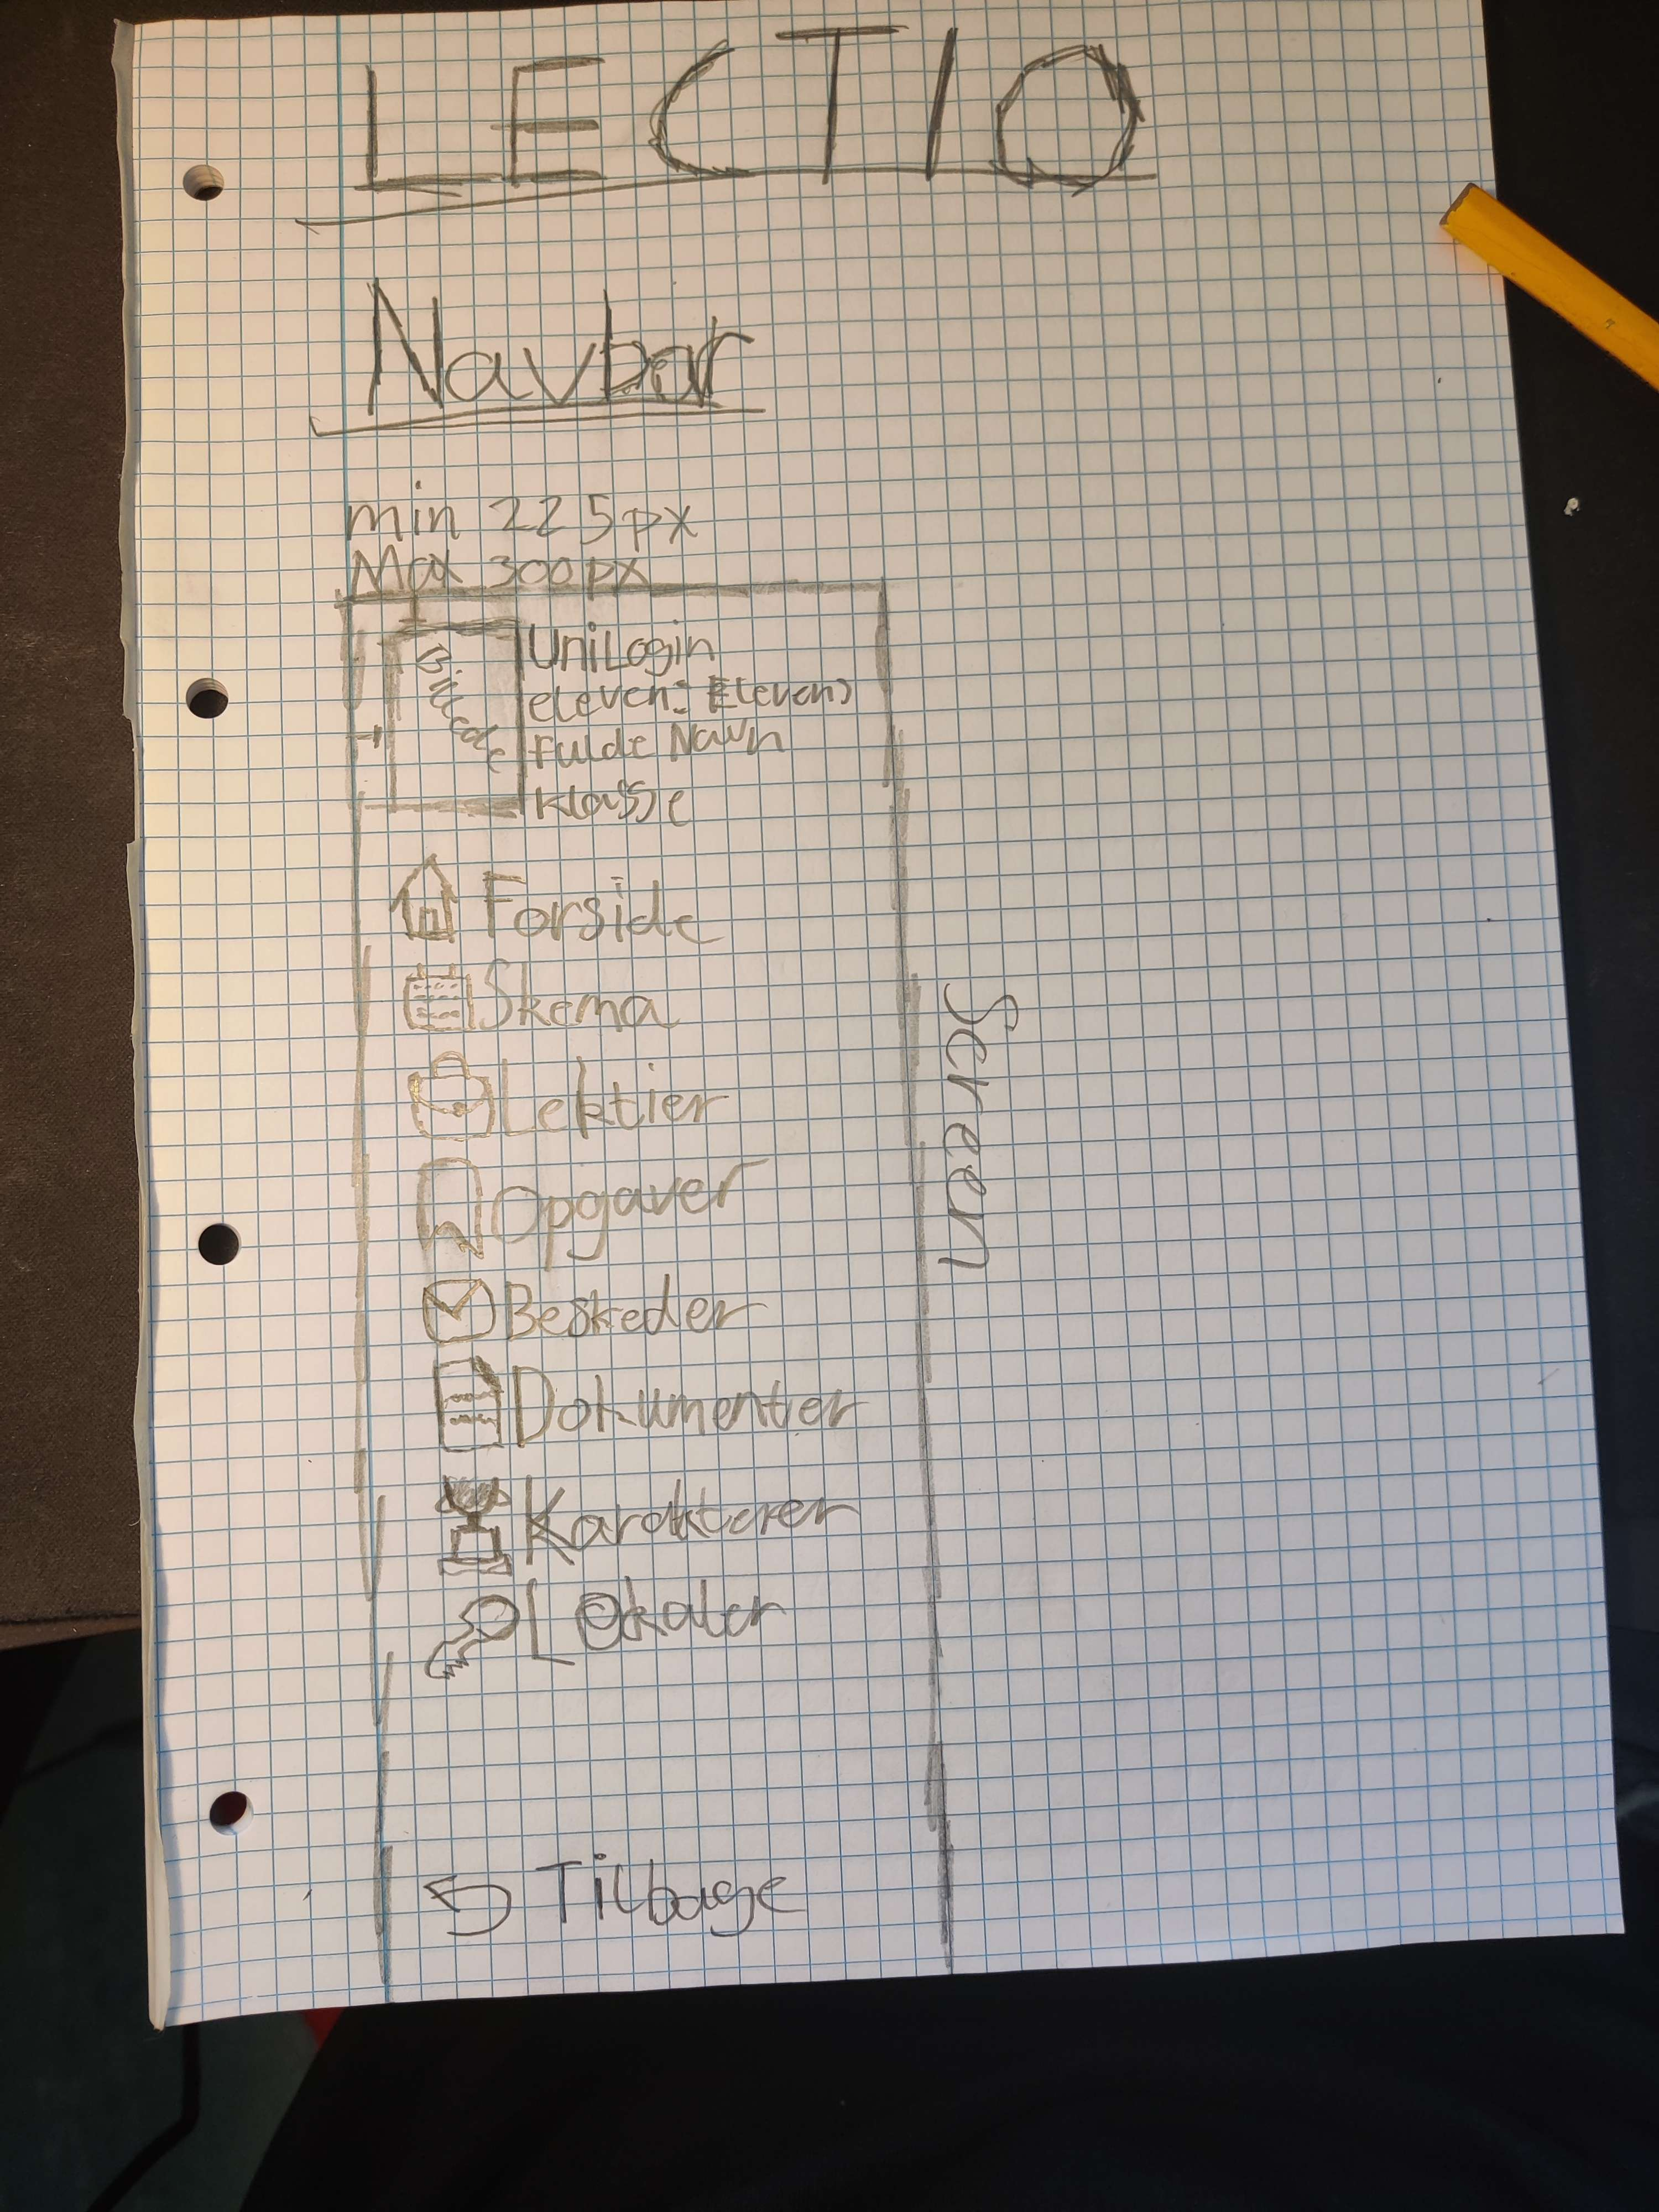
\includegraphics[]{assets/lectio_navbar_skitse.jpg}}
            \caption{Viser Lectioreworkets navigationsbarkomponent - bjælken, brugeren intergerer med}
        \end{figure}

        \begin{figure}[H]
            \centering
            \resizebox{!}{10cm}{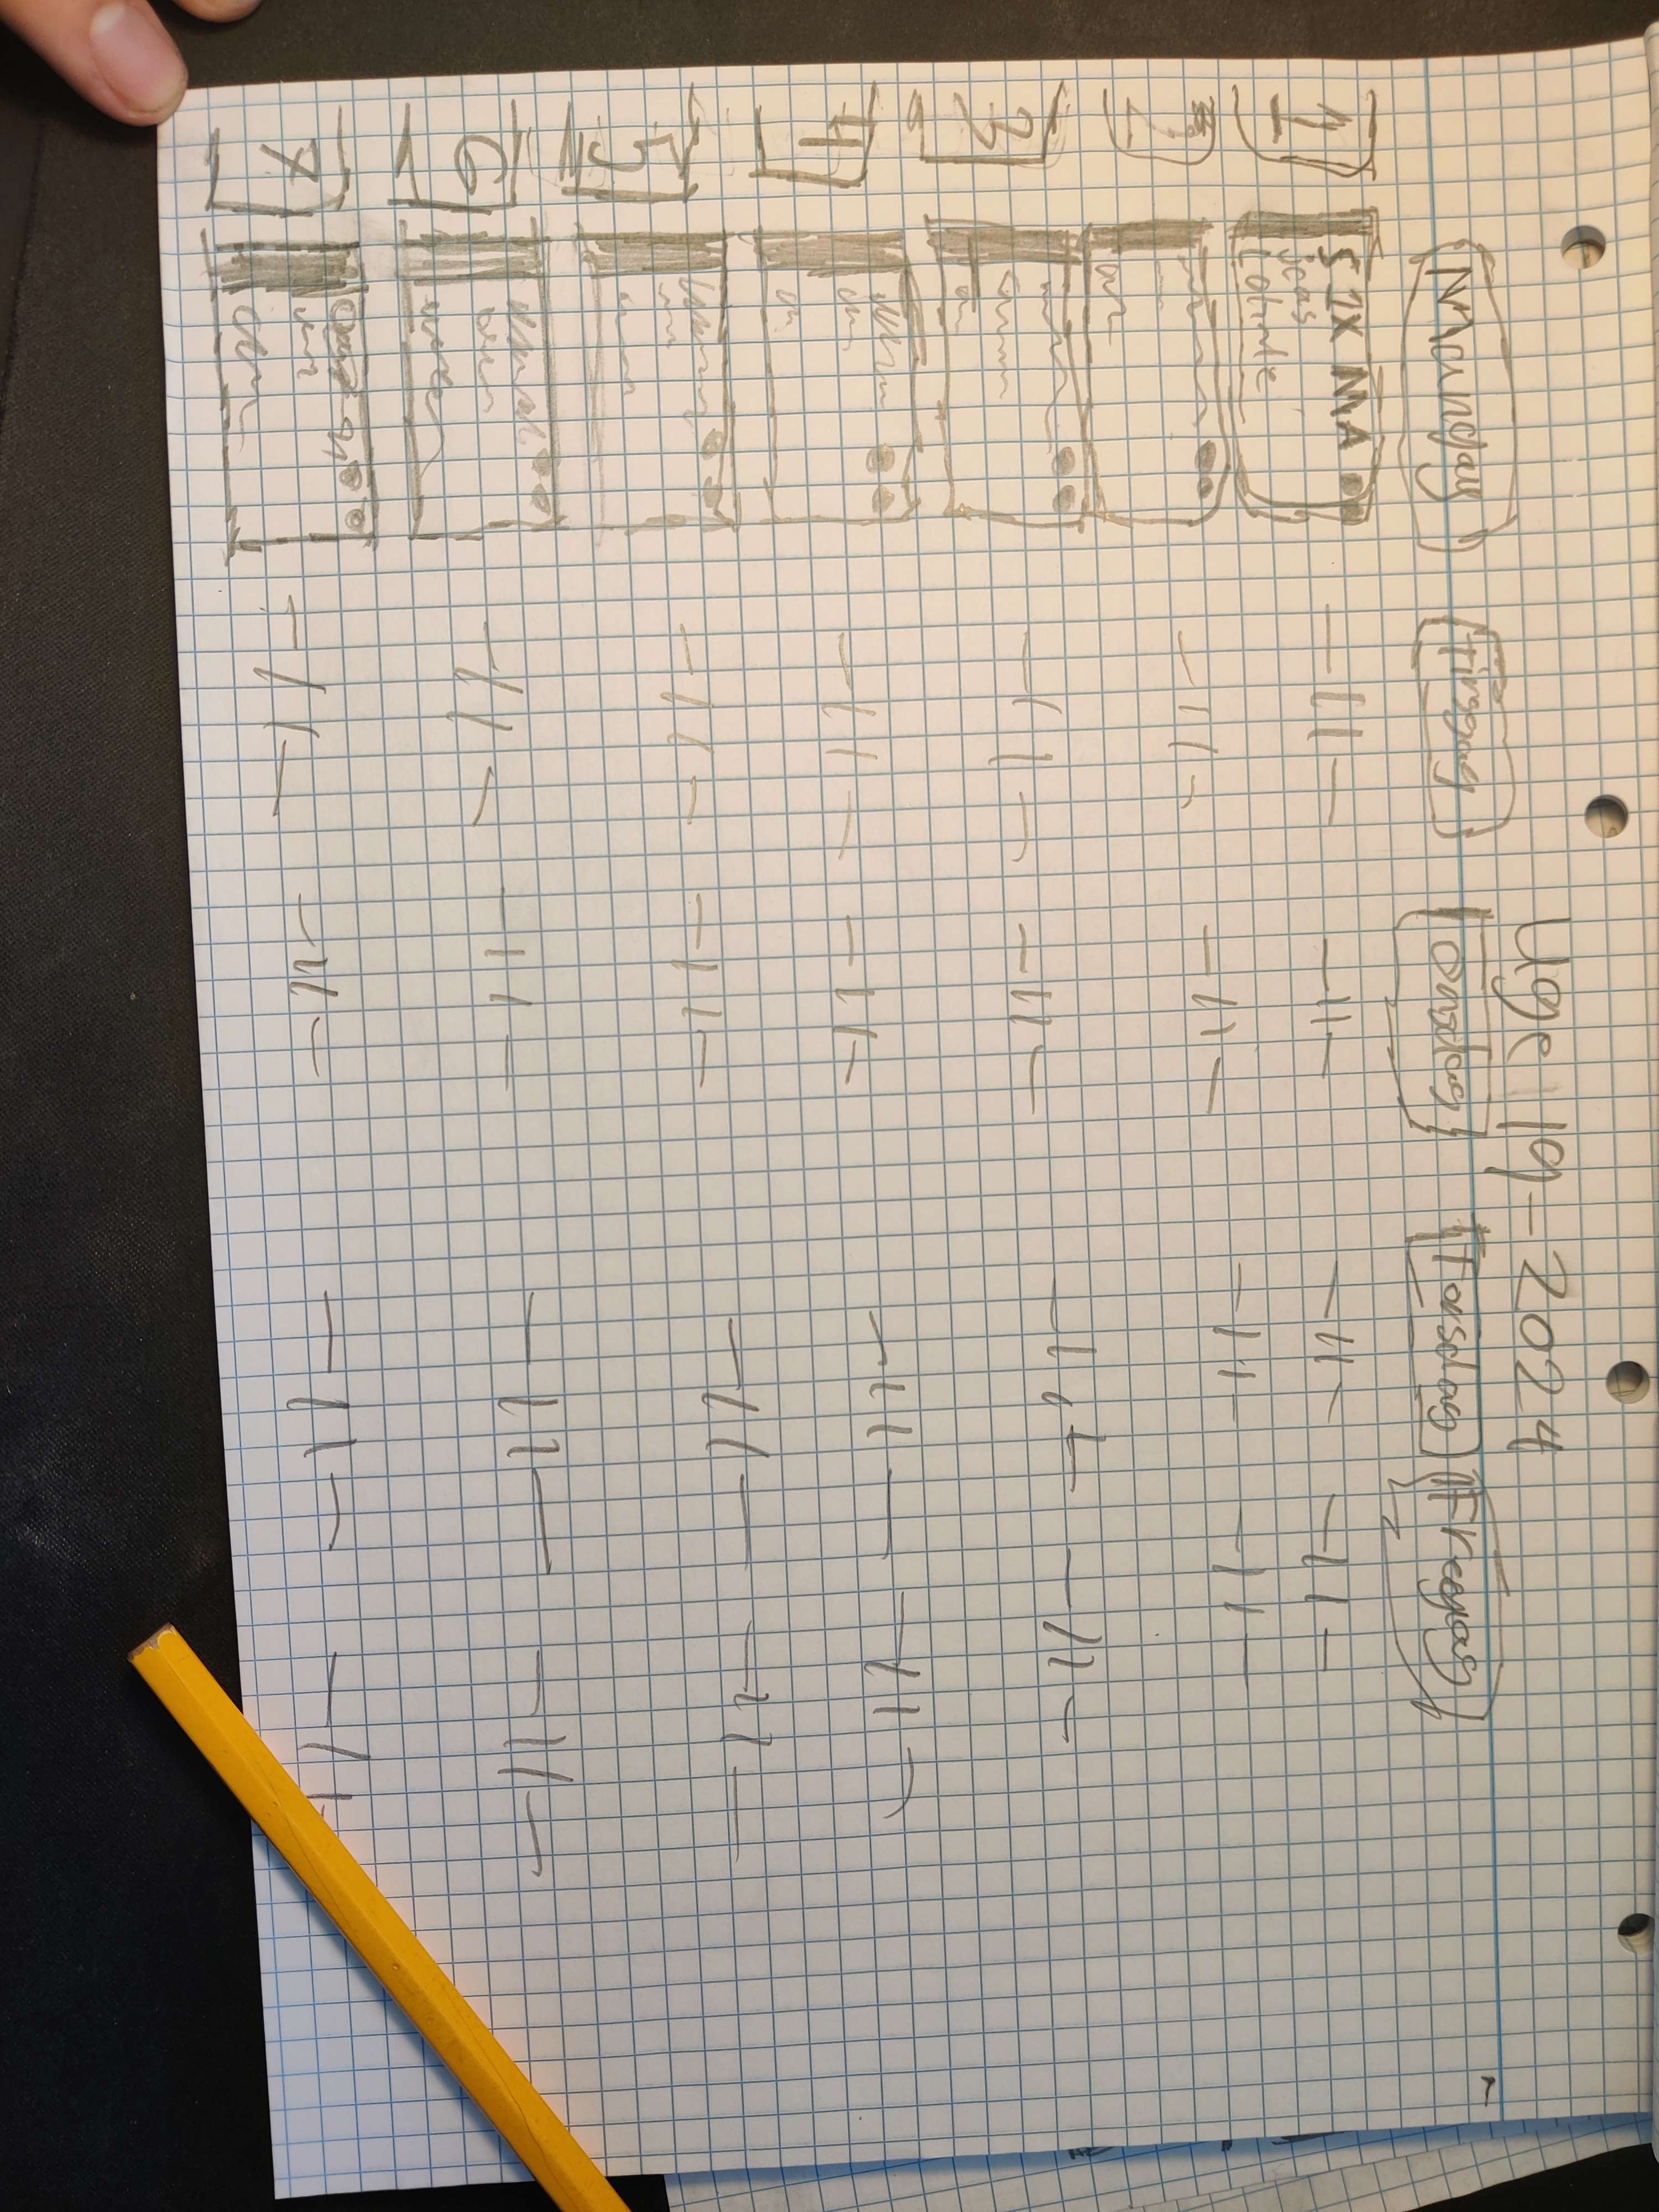
\includegraphics[angle =90]{assets/lectio_skema_skite.jpg}}
            \caption{Viser Lectioreworkets skema side}
        \end{figure}

        De resterende skitser, vi har udarbejdet, fremgår af appendikssektionen \ref{appendix:arbejdsskitser}.

        \subsubsection{RFID-Løsning}
        For at tage hånd om problemet med spildtid i form af fraværstagning, fejlagtig fraværstagning m.v. har vi valgt at lave et dør/fraværssystem, som når man om morgnen møder ind, scanner man sig ind med sit ID-kort eller sit
        digitale ID-kort med sin mobiltelefon på fraværsregistreringssystemet som er i klassen.  
        Lokale-Booking-Systemet fungerer (i ideen--se evalueringen \ref{sec:konklusion}) i sammenspil med den nye Lectio applikation, så kan igennem applikationen booke et lokale også med sit ID-kort
        låse lokalet op i det tidsrum man har booket det pågældene lokale. Web løsningen ses skitseret forneden:

        \begin{figure}[H]
            \centering
            \resizebox{!}{10cm}{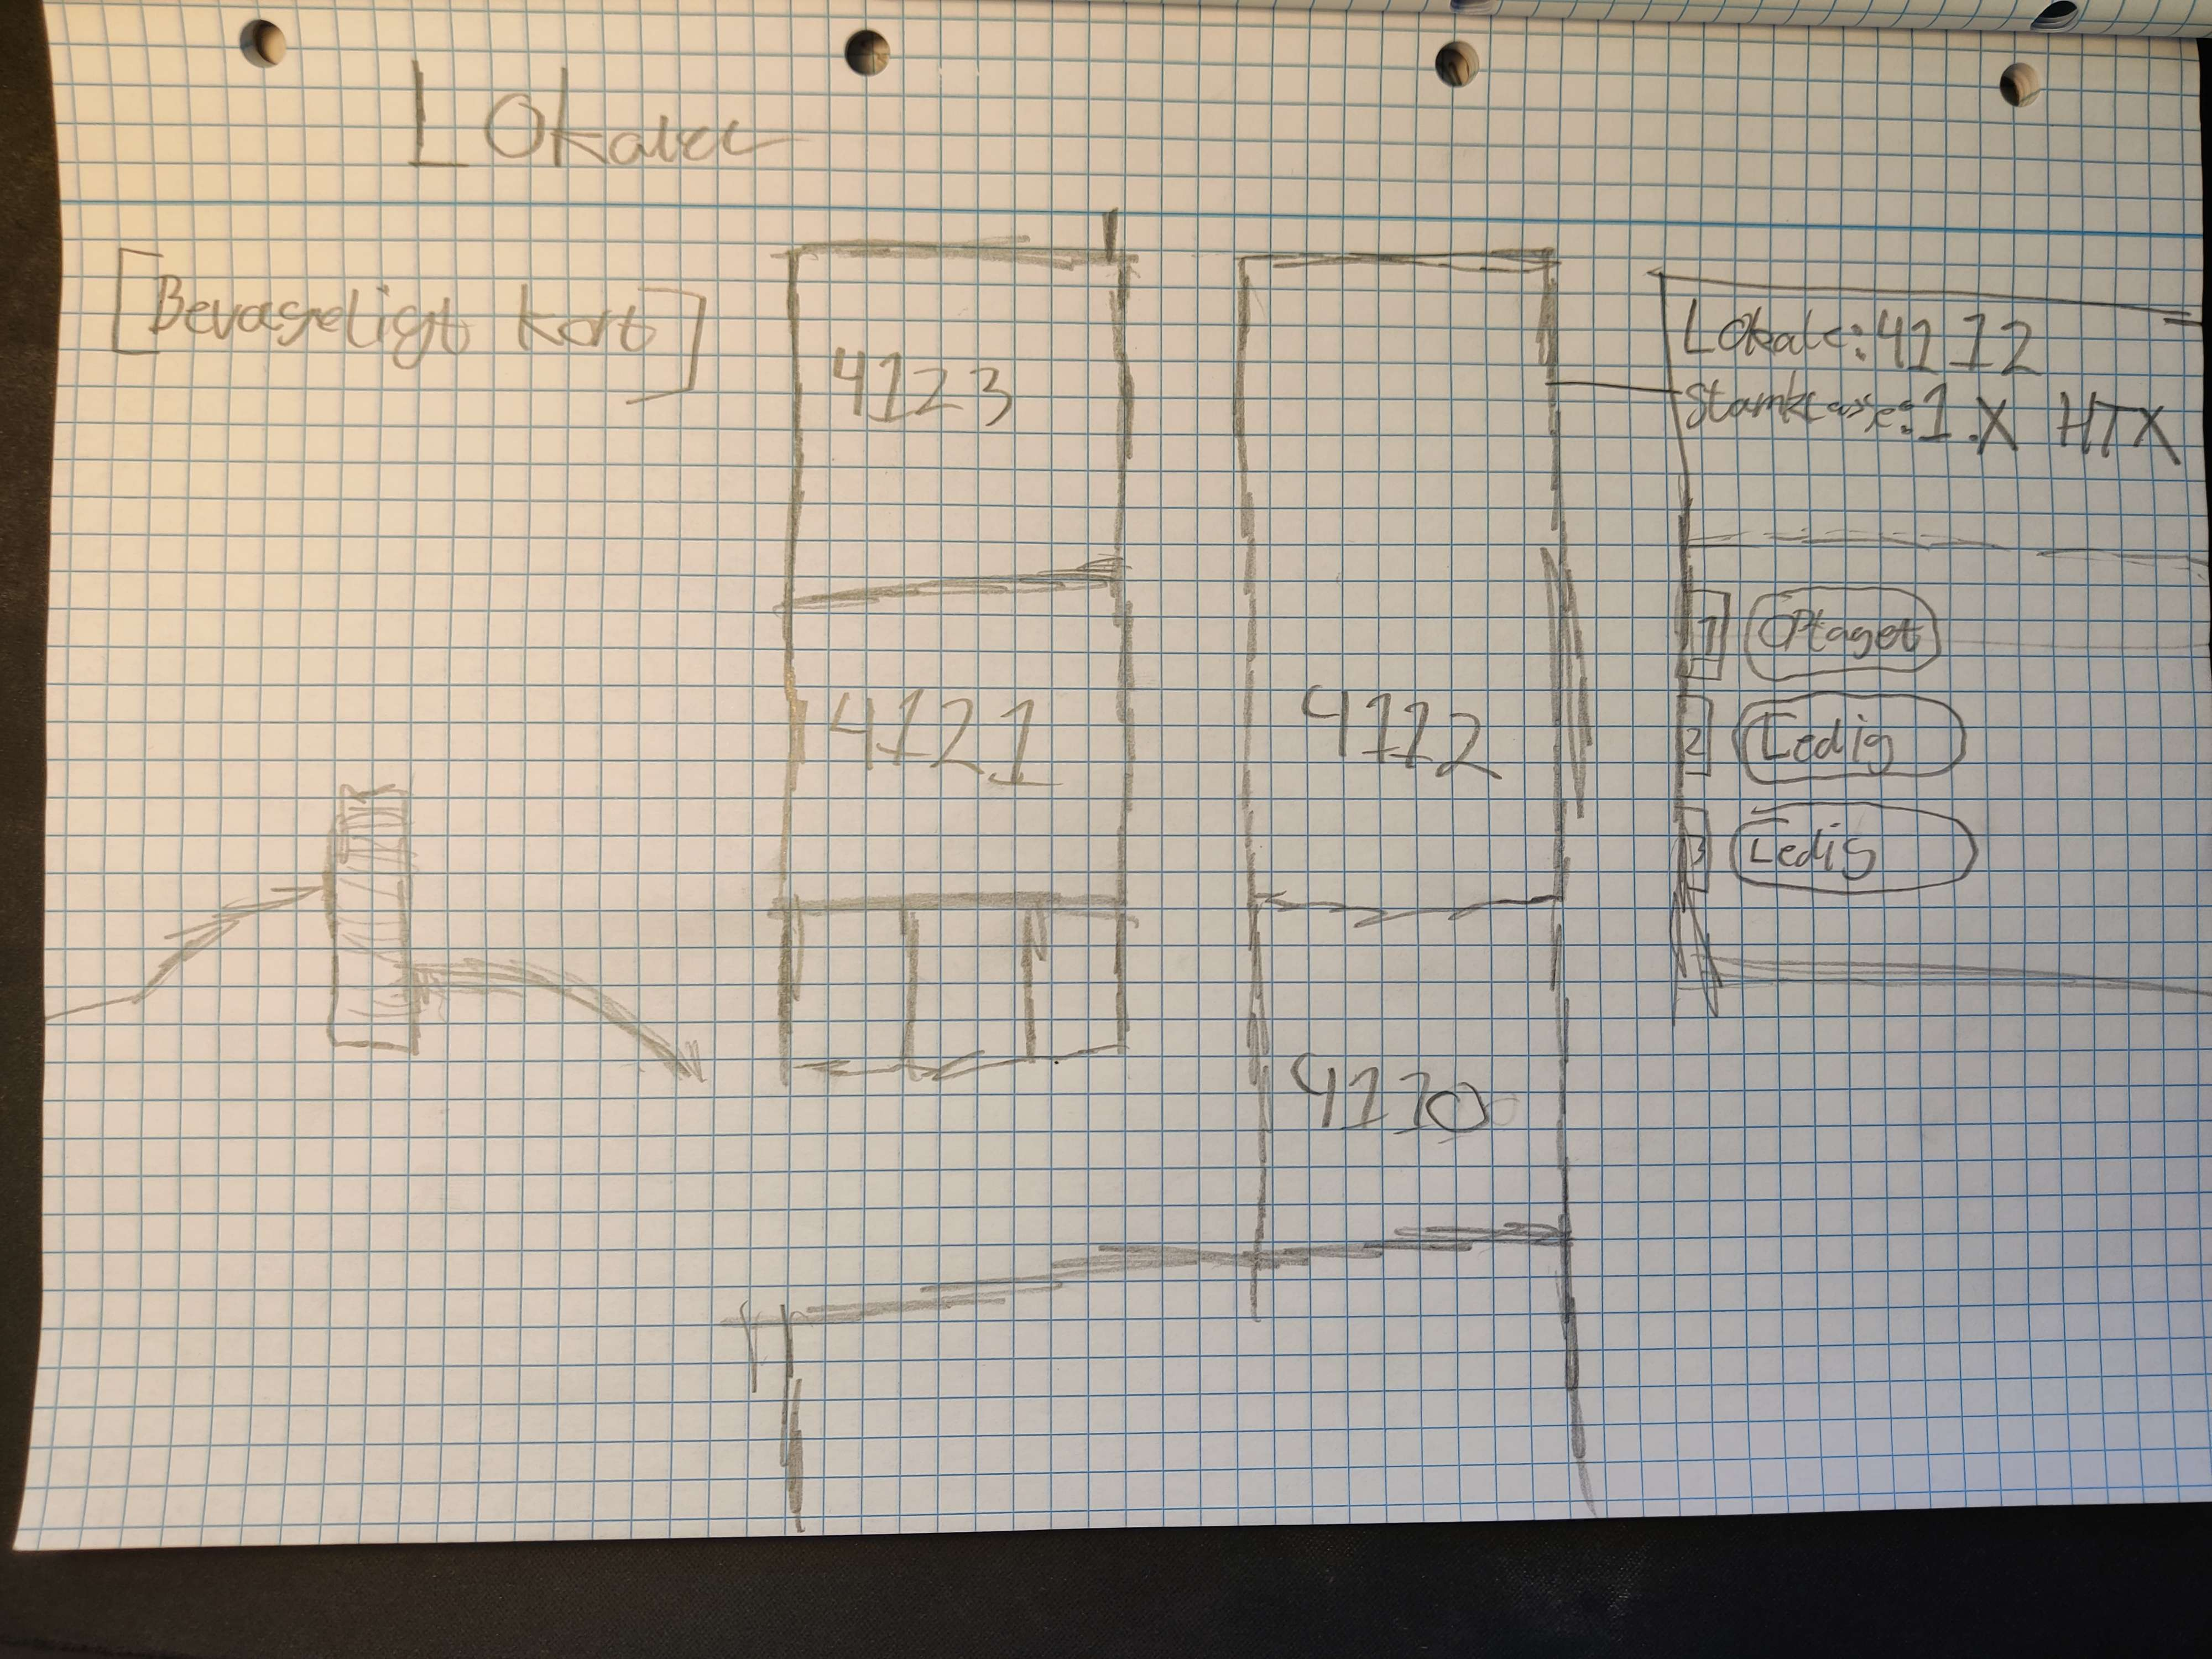
\includegraphics{assets/lectio_lokaler_skitse.jpg}}
            \caption{Viser Skitse af Booking siden på samme webapplikation som Lectio Reworket}
        \end{figure}
         \newpage
    \section{Produktudformning \label{sec:produktudformning}}
    \subsection{Lectio rework}
        \subsubsection{Overordnet}
           Lectio-applikationen er skrevet i et populært framework, Next.js, som er en overbygninng på React-biblioteket til node.js, der tillader at man kan køre javascript på en server i stedet for i Chrome V8-motoren, som kun tillader at man køre javascript clientsided fremfor serversided.

            React er et library for user interfaces, der tillader UI-komponenter, der i sammenspil med HTML, udgør en brugeroverflade. HTML står for >>HyperText Markup Language<<, der er standard markupsproget til alle hjemmesider--alt indhold, der serveres på internettet. Et markupsprog, fx. \LaTeX, som dette dokument er skrevet i, i modsætning til programmeringssprog, anvendes til at overlevere informationer til mennesker--programmeringssprog anvendes til at give instrukser til computere.

           Selve renovering er rent faktisk en renovering i den forstand, 
           at den reelle hjemmeside er blevet forbedret eller fornyet, 
           men derimod er den blevet genopygget fra bunden af dog med henblik på at bevare den samme funktionalitet. 
           Af den grund er det en mere korrekt betegnelse at kalde det et >>rework<<.
        \subsubsection{Kodegennemgang}
        Forneden er en komplet gennemgang af koden til Lectio-reworket.       

        En filstruktur behøver æstetisk, letoverskuelig og forståelig både i menneske- og computertermer.
        Således er der både de prædefinerede valg og de mere artistiske valg. 

        Et Next.js-projekt (v.14) benytter deres nyligt lancerede app router-filstruktursystem, således skal filer struktures på følgende vis: man har >>Top-level files<<, der bruges til applikationkonfiguration, administration af filafhængigheder m.m.\cite{projstruct}
        \begin{figure}[H]
        \dirtree{%
            .1 /.
            .2 {\color{blue}{app}}.
            .2 jsconfig.json.
            .2 LICENSE.
            .2 next.config.js.
            .2 {\color{blue}{node\_modules}}.
            .2 package.json.
            .2 package-lock.json.
            .2 postcss.config.js.
            .2 {\color{blue}{public}}.
            .2 REDME.md.
            .2 tailwind.config.js.
           }
        \caption{Top-level filstrukturen for lectio-reworket. Mapperne er farvet blåt}
        \label{fig:tlprojstruct}
        \end{figure}

        Forneden gennemgås top-level filerne og mapperne efter hensyn til forståelsen, der fremgår af figur (\ref{fig:tlprojstruct})

        \paragraph{next.config.js} er en konfigurationsfil for Next.js, der tillader, at man konfigurer sprogets funktionalitet. 
        
        \paragraph{LICENSE-filen} er en fil, der indeholder projektets licens og brugsrettigheder, og da vores er et open source-projekt (open source vil sige, at alle kan tilgå det "gratis"), så bruges MIT-licensen, der tillader al brug af materialet til alle formål af alle individer. 
        
        \paragraph{jsconfig.json} er en projektafhængighed for javascriptsproget, og den indeholder kompileringsvariabler, få. 

        \paragraph{tailwind.config.js. \label{par:tailwind}} er en konfigurationsfil, der konfigurer CSS. CSS er et understøttende design systemssprog til HTML, så alt der har med design at gøre, dvs. tekststørrelser, farver mv. "styles" i CSS. I Lectio.v2-applikation anvendes Tailwind-CSS, et framework til CSS, til at style dette; det er lettere overskueligt, hurtigere og standardiseret. Se forneden kode og rendering\ref{fig:modulbrikfostaaelse}:
        \begin{figure}[H]
            \begin{lstlisting}[language=HTML]
<div className="bg-[#9CCEFF] 
    border-l-[10px] 
    border-l-[#1E90FF] 
    p-4 
    rounded-lg 
    max-w-[275px] 
    max-h-[88px] 
    flex 
    justify-between 
    cursor-pointer 
    hover:opacity-80 
    group">

<div className="flex flex-col text-[#0D3F70] justify-center">
    <span className="font-bold text-xl">S 1x { args.subject }</span>
    <span>{ args.teacher }</span>
    <span>{ args.room }</span>
</div>    
            \end{lstlisting}
            \begin{center}
            
\includegraphics{assets/moduleElement.png}
            \end{center}
            \caption{Viser en modulbrik m. tilhørende CSS-kode (notér at dette ikke er den komplette kode [tjek bilag \ref{appendix:modulbrikkode}] til brikken, dog godt nok for at illustrere vores pointe) \label{fig:modulbrikfostaaelse}}
        \end{figure}
        \paragraph{app-mappen overordnet \label{pgh:app-ov}} indeholder reworkets reelle koder, i modsætning til de andre filer, der primært konfigurer koden og den gør kørbar. 
        Neden for ses hvordan vi har struktureret app-mappen. 
        \begin{figure}[H]
            \dirtree{%
                .1 app.
                .2 page.jsx.
                .2 layout.jsx.  
                .2 {\color{blue}{dashboard}}.
                .3 layout.jsx.
                .3 page.jsx.
                .2 {\color{blue}{lokaler}}.
                .3 page.jsx.
                .2 {\color{blue}{skema}}.
                .3 page.jsx.
                .3 skema.json.
                .3 {\color{blue}{[slug]}}.
                .2 {\color{blue}{ui}}.
                .3 {\color{blue}{dashboard}}.
                .3 {\color{blue}{navbar}}.
                .3 {\color{blue}{skema}}.
                .3 globals.css.
               }
            \caption{Filstrukturen for app mappen. Mapperne er farvet blåt}
            \label{fig:app-mappen}
            \end{figure}
        I Next.js, er alle mapper i /app-mappen, det er et subdomain, når det indeholder en >>page.jsx<<-fil. Men hvad er et subdomain? Før vi kan forstå det, skal vi se på, hvad er en URL? URL står for 
        Uniform Resource Locater. En URL er struktureret med først en protokol, som for web ressourcer er enten HTTP (Hypertext Transfer Protocol) eller HTTPS (HTTP Secure). Andre protokoller inkludere f.eks. FTP som er en >>File Transfer Protocol<<  
        efter protokollen kommer domænenavnet. Domænenavnet referer til en ip-adresse.  Det vil sige, at når man søger efter et domænenavn, søger man i en DNS-server (Domain Name System) og finder den tilknyttede ip-adresse,
        som sender den data, som hjememsiden består af til browseren. Efterfølgende kan der være subdomains der er alt efter domainenavnet plus et /.

        \begin{figure}[H]
        \begin{mdframed}
        \begin{equation*}
        \stackrel{\text{Internetprotokol}}{\overline{\text{https}}}:// \stackrel{\text{domænenavn}}{\overline{\text{noget.dk}}} / \stackrel{\text{subdomæne}}{\overline{\text{nogetandet}}}
        \end{equation*}
        \begin{center}
            Uniform Ressource Locater
        \end{center}
        \end{mdframed}
        \caption{Viser opbygningen af en URL}
        \end{figure}
        \newpage
        
        \paragraph{package.json} indeholder modulafhængigheder, der er hentet via NPM (Node package manager), der udnytter node.js. Forneden er et udsnit fra dette, der viser >>dependencies<<:
        \begin{lstlisting}[language=Javascript]
"dependencies": {
    "@heroicons/react": "^2.0.18",
    "@vercel/postgres": "^0.5.1",
    "bcrypt": "^5.1.1",
    "current-week-number": "^1.0.7",
    "dotenv": "^16.3.1",
    "heroicons": "^2.0.18",
    "next": "14.0.3",
    "react": "^18",
    "react-dom": "^18",
    "react-draggable": "^4.4.6"
    }, 
        \end{lstlisting}

        Mod venstre kan man se navnet på NPM-pakken. Efter kolonnet til højre ses versionen af denne. Næsten alle dem, der fremgår, bliver udnyttet, dog er der få som blot er resultatet af skabelonbrug. Denne skabelon er tiltænkt til fremtidig brug, så den kan anvendes til flere formål. Skabelonen kan også tilgås via GitHub.

        Her er en kort gennemgang af nogle af pakkerne, der er hentet via NPM, som vi bruger, der tilføjer ekstra funktionalitet:
        \begin{itemize}
        \item heroicons - Anvendes forskellige steder i koden, hvor ikoner anvendes. Heroicons fungerer således, at ønskede ikoner kan importeres fra heroicon-bibliotektet, hvorefter de kan indsættes i web-applikationen
        \item current-week-number - Anvendes til at fremkalde det nuværende ugetal via en applikation programm. Det i vores tilfælde til at indsætte ugetallet i skemabrikken. 
        \end{itemize}

        \paragraph{app-mappen}
            Vi startede med at gennemgå overordnet app-mappen (\ref{pgh:app-ov}), her er en dybdegående genemgang. App-mappen består af subdomænemapper og en UI-mappe (user interface).
            
            UI-mappen består af komponenter, fx. navigationsbaren, der anvendes på diverse web pages. Heraf er nogle af disse komponenter konsekvente på alle webpagesne, hvorfor det ikke giver mening at genskrive dem i hvert subdomæne. Disse konsekvente komponenter har ophav i root-layout.jsx mappen.
        
            \subparagraph{Layout.jsx-filen}
            \begin{figure}[H]
                \dirtree{%
                    .1 app.
                    .2 page.jsx.
                    .2 {\color{red}{layout.jsx.}}.
                    .2 {\color{blue}{dashboard}}.
                    .2 {\color{blue}{lokaler}}.
                    .2 {\color{blue}{skema}}.
                   }
                \caption{Filstrukturen for app mappen. Mapperne er farvet blåt}
                \begin{lstlisting}[language=Javascript]
import './ui/globals.css';
import { Inter } from 'next/font/google'
import Navbar_client from './ui/navbar/navbar-client'
import Navbar_server from './ui/navbar/navbar-server'

const inter = Inter({ subsets: ['latin'] })

export default function Layout({ children }) {

    return ( 
        <html lang="en">
            <body className={`${inter.className} antialiased flex justify-start`}>
                <Navbar_client>
                    <Navbar_server />
                </Navbar_client>
                {children}
            </body>
        </html> 
        );
}
                \end{lstlisting}
                \caption{Viser hvor layout.jsx (markeret rød) befinder sig i projektets filstruktur samt dens inhold \label{fig:layout}}
            \end{figure}
            Den importerer navbaren på klient- og serverside, hvorefter denne renderes, hvilket resulterer i, at den ikke behøves genrenderes hele websittets livscyklus.

            Måden, hvorpå navbaren forbliver det samme sted på div. webpages, er ved, at layout-filen agerer en overordnet skabelon, hvorefter subdomænernes og forsidens pagefils kode tilføjes under pladsholderen {children}.
            Se figur (\ref{fig:layoutforståelse}) nedenfor for forståelse.

            \begin{figure}[H]
                \centering
                \fbox{\resizebox{\columnwidth}{!}{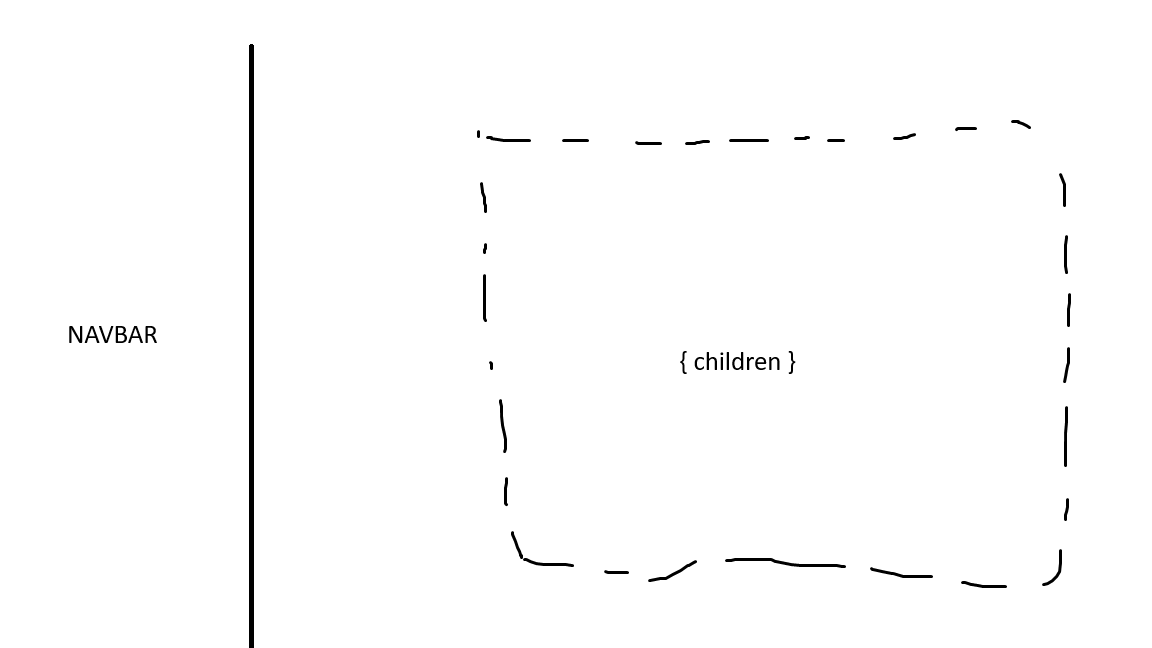
\includegraphics{assets/layout.png}}}
                \caption{Viser, hvordan layoutfilen påvirker webpagesnes rendering. \label{fig:layoutforståelse}}
            \end{figure}

            \subparagraph{page.jsx-filen}
            Page.jsx-filen er hjemmesidens forsidefil; det første forbruger møder. Page.jsx-filen indeholder tre primære HTML-sektioner (<div>), der på brugeroverfladen fremstår som kasser; som igen er stilet med CSS-tailwind (se paragraf \ref{par:tailwind}).

            \subparagraph{Skemakoden}
            Skemakoden er den del af Lectio-applikationen, vi har brugt mest tid på, da denne også dag-til-dag er vigtigst samt involverer databaseinfrastruktur. 
            
            Koden kan nedbrydes til dage, der kan nedbrydes til moduler. Dagene består et array (liste), hvor hvert et element i arrayet (listen) er et kodeobjekt, der indeholder modulsinformation, herunder faget, underviseren, lokation (lokale), noter, lektier samt metadata som synlighed (om folk skal se dig). Envidere indeholder det også et autogeneret ID, der anvendes til autogeneret web pages, der viser detajleret information om det individuelle modul.
            \begin{figure}[H]
                \begin{lstlisting}[language=Javascript]
// Monday
const scheduleMon = [
    { subject: 'MA', teacher: 'jacs', room: 'SLWI-4110', id: '1fxh', 
    visibility: 'show', note: 'Plan: Potensfunktioner, eksponentiel vaekst', homework: '03_opg_polynomier.ipynb' },
    
    { subject: 'MA', teacher: 'jacs', room: 'SLWI-4110', id: '123afa', 
    visibility: 'show', note: '', homework: '' },
    
    { subject: 'Fy', teacher: 'hnpo', room: 'SLWI-4110', id: 'qw123ac', 
    visibility: 'show', note: 'Ingen lektier. Vi ser paa hvad vi skal i timen. Forberedelse til SO2 i naeste uge. we  we jwnkjnkjn kjnkjnkjn ', homework: '' },
    
    { subject: 'Fy', teacher: 'hnpo', room: 'SLWI-4110', id: 'xcv12', 
    visibility: 'show', note: '', homework: '' },
    
    { subject: 'sa', teacher: 'mmje', room: 'SLWI-4110', id: 'sdvf23', 
    visibility: 'show', note: 'Det senmoderne samfunds kendetegn ', homework: '' },
    
    { subject: 'So', teacher: 'kibo', room: 'SLWI-4110', id: 'sdf123', 
    visibility: 'show', note: '', homework: 'Hold 'o'je med, hvordan du tager noter i de forskellige fag.' },
    
    { subject: '', teacher: '', room: '', id: 'sdv135', visibility: 'hide', note: '', homework: '' },
];
                \end{lstlisting}
                \caption{Viser et eksempel koden, der skal til for en dag. \label{fig:dataeksempel}}
            \end{figure}

        Alle dagene har et tilsvarende array med objekter. Selve skemaet er en kodetabel, der består af rækker (tablerowelement). SkemaModule-komponentet tager imod argumenter, hvilke hentes fra den tidligere sete kode. 
        \begin{figure}[H]
        \begin{lstlisting}[language=Javascript]
<td><SkemaModule subject={scheduleMon[0].subject}
<td><SkemaModule subject={scheduleTue[0].subject}
<td><SkemaModule subject={scheduleWed[0].subject}
<td><SkemaModule subject={scheduleThu[0].subject}
<td><SkemaModule subject={scheduleFri[0].subject}
        \end{lstlisting}
        \caption{Viser at >>SkemaModule<<-komponentet tager første (nulte i kode) objekt i schedule<dag>'s kodeproperty (properties er en værdi, der tilhører et objekt). SkemaModule modtager langt flere properties fra de respektive objekter, fx lærer, fag osv.; dett er et udsnit--se appendiks \ref{appendix:SkemaModule} for resterende kode.}
        \end{figure}
       
        \subparagraph{SkemaModule.jsx}
        SkemaModule.jsx-filen indeholder det komponent, der referers tidligere >>SkemaModule<<, heri bliver argumenterne indsat i HTML-kode, hvor der et script, der tjekker om args.note er tom, altså om der er lektionnoter, for det pågældende modul--hvis denne ikke er tom (altså \textit{indeholder}), viser den et ikon, og det samme sker med args.homework, således at "lektieikonet" vises. Ligeledes dukker "tooltips" også op, når brugerens mus er over et modulelement, dog udover at der tjekkes om argumenterne/propertiesne er tomme, importeres værdien og renderes i selve tooltippet. Se figur for forståelse:

        \begin{figure}[H]
        \centering
        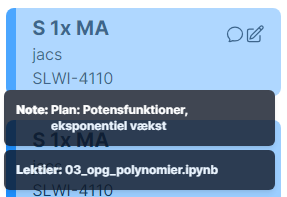
\includegraphics{assets/moduleElement2.png}
        \caption{Viser et modul, hvis args.note og args.homework-argumenter/properties ikke er tomme samt har værdier; ligeledes de respektive tooltips og ikoner.}
        \end{figure}
        
        \subparagraph{Datohåndteringssystem}
        Datahåndteringssystemet fungerer på den måde, at der op i toppen defineres et array med datoer, dette er datoerne, der fremgår på vores skemaeksempel; hvis softwaren skulle distribueres ville disse blive indhentet via en API (Application programming interface), således datoerne bliver dynamisk opdateret.

        Forneden fra linje 4-10 indhentes dagens dato, hvorefter denne anvendes til at skrive dags dato. Herefter laves en konstant, der tager variablerne >>date<< og >>month<<, disse anvendes senere ned til at blive sammenlignet med >>Current 
        \begin{lstlisting}[language=Javascript]
const weekNumbers = ["29/4", "30/4", "1/5", "2/5", "3/5"];


const today = new Date();
const month = today.getMonth()+1;
const year = today.getFullYear();
const date = today.getDate();
const currentDate = month + "/" + date + "/" + year;

const currentFormattedDate = month + "-" + date + "-" + year; 

const weekDate = date + "/" + month;

var currentWeekNumber = require('current-week-number');

// Her er en masse kode imellem se appendiks F

{ (() => {
    if (weekNumbers[0] == weekDate) {
        return (
            <span className="px-10 p-4 rounded-xl bg-[#1E90FF] text-white font-normal">Mandag <strong>{ weekNumbers[0] }</strong></span> 
        );
    } else {
        return (
            <span className="px-10 p-4 rounded-xl bg-slate-200 font-normal">Mandag <strong>{ weekNumbers[0] }</strong></span>
        );
    }

})()}
        \end{lstlisting}
    Herefter tjekker koden om den pågældende ugedag er lig med dags dato, hvorefter dennes respektive UI-element i så fald gøres blåt for at indikere til brugeren, at denne dad er dags dato.
    
    \subparagraph{Dynamic Routes (slugs)}
    Dynamic routes er "ruter" til data, hvis specifikke lokation vi ikke kender i forvejen (generer subdomæner dynamisk ud fra input). Dynamic routes anvendes i dette tilfælde til automatisk generation af sider med et respektivt moduls deltajeret information og oversigter, herunder vehæftelser. 
    Denne genereres ved, at der i skemasubdomænet eksisterer et subsubdomæne med square brackets herom [], hvilket fortæller dokumentet er der er tale om et dynamisk sub(sub)domæne, hvori der ligger en page.jsx-fil tilsvarende til dem, vi har gennemgået tidligere, dog er denne 100\% dynamisk, og der specificeres, hvordan information skal formateres, men selve informationen / indholdet hentes via et API fra en anden webserver / serverdatabase. Datasvaret, vi ville få, er samme type som vores skemakoder anvender (objekter), ergo næsten ens, da dette også er .JSON-format--se tidl. figur for dataeksempel \ref{fig:dataeksempel}. 
        \begin{figure}[H]
        \centering
        \resizebox{\columnwidth}{!}{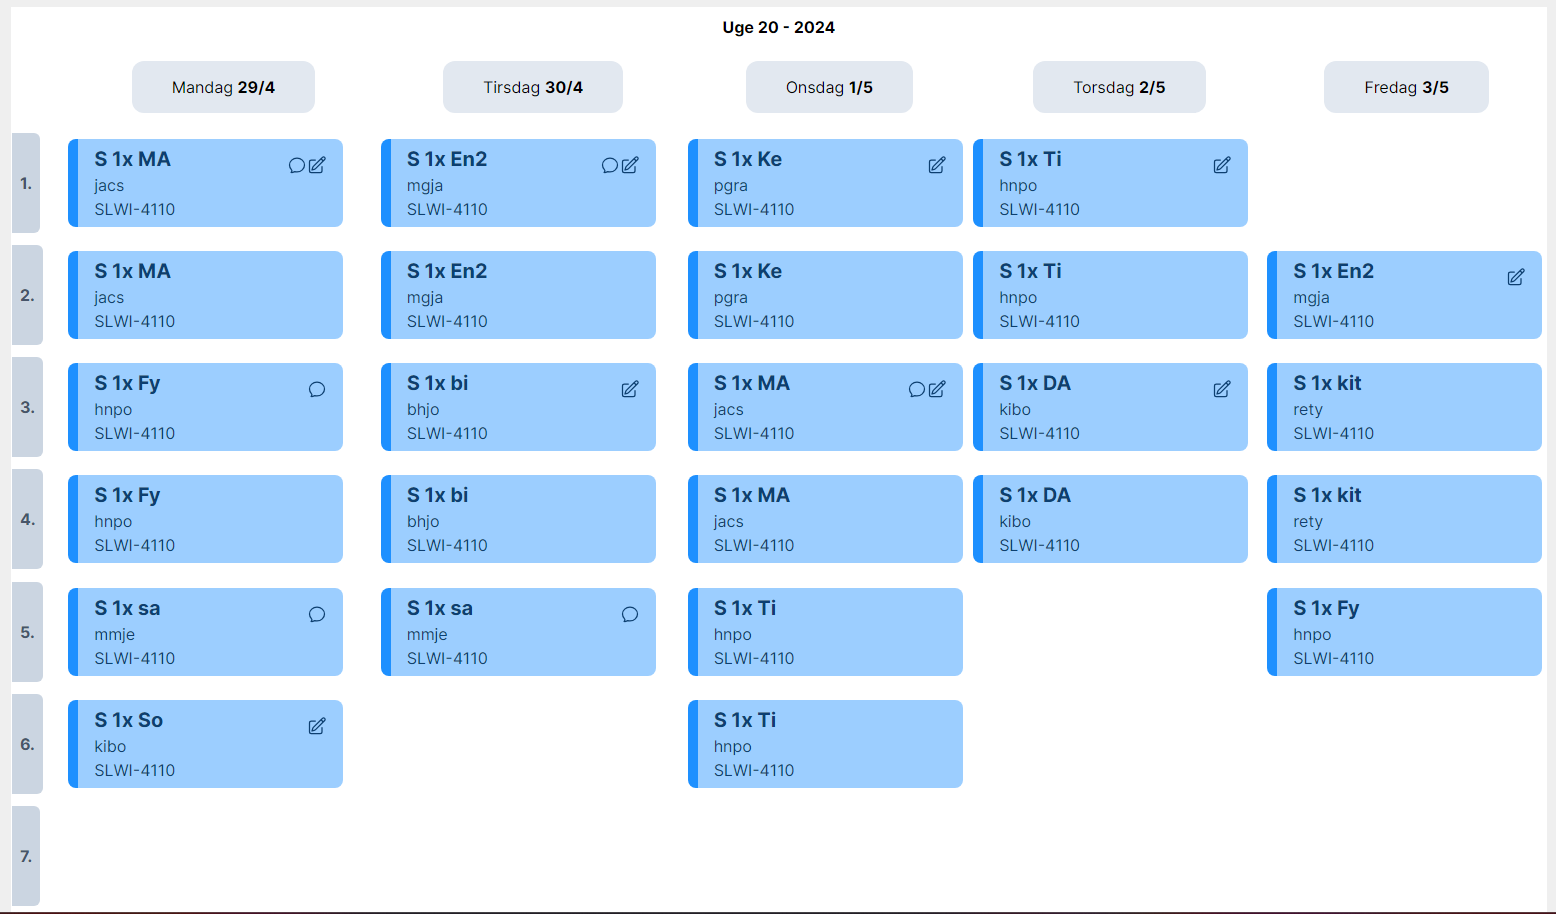
\includegraphics{assets/skemaElement.png}}
        \caption{Viser skemaet.}
        \end{figure}
\subsection{Bookingsystem}
    Vi har valgt at fjerne bookingsystems-delen for dette produkt; dog er den skidegod ide, og det var blevet en del af produktet. Det er af rent pragmatiske årsager, at vi vælger ikke at udvikle systemet, det havde garanteret været sjovt. Skitserne over dette fremgår af appendiks \ref{appendix:arbejdsskitser}.

\subsection{RFID-System}
    \subsubsection{Overordnet}
    Som del af vores teknologiprojekt fandt vi frem til at vi kunne forbedre studiemiljøet ved at implementere døre på skolen der benytter sig af RFID (Radio-frequency identification). 
    Og udlevere studiekort til elever som de kan benytte sig af til f.eks. at åbne bookede lokaler eller til hurtigere at tage fravær,
    og i tilfælde af brand ville der også være mulighed for at låse alle døre op til potentielle flugtveje. disse er alle ting som er med til at modernisere IT-Infrastrukturen på skolen, 
    og derved forbedre studiemiljøet for elever.

    \subsubsection{Konstruktion}
    Da vi gik i gang med at planlægge konstruktionen af produktet kom vi ret hurtigt frem til at det ikke ville være en mulighed at bygge en dør med scanneren på, vi besluttede derfor at,
    vi ville konstruere en primitiv prototype i stedet for, som en form for repræsentation af hvad det rigtige produkts egenskaber ville være. vi har dog lavet alle overvejelserne til det rigtige produkt.
    den prototype er placeret i en gammel kasse vi havde, da det stadigvæk fint repræsenterer funktionaliteten af produktet, inde i kassen er der et stort breadboard, esp-wroom32 (devkitC variant),
    en lille powersupply der bruger et lithium-ion batteri, 2 led'er, og en RFID-RC522 scanner. disse komponenter er alt der der skal til for at få selve hardware delen til at virke. 
    for at korrekt sammensætte disse komponenter fulgte vi dokumentationen for RFID-RC522 scanneren som vi fandt online, efterfølgende tilføjede vi de ting der skulle til for at få prototypen til at repræsentere
    det vores produkt skulle kunne. opsætningen af esp32'eren var lidt udfordrene men fandt heldigvis nogen guides der beskrev nogle hovedpunkterne i forhold til opsætning.
    
    men før vi gik i gang med at bygge selve kassen havde vi lavet et diagram i EasyEda der viste hvordan at prototypen ville komme til at se ud.'
    
    \begin{figure}[H]
        \centering
        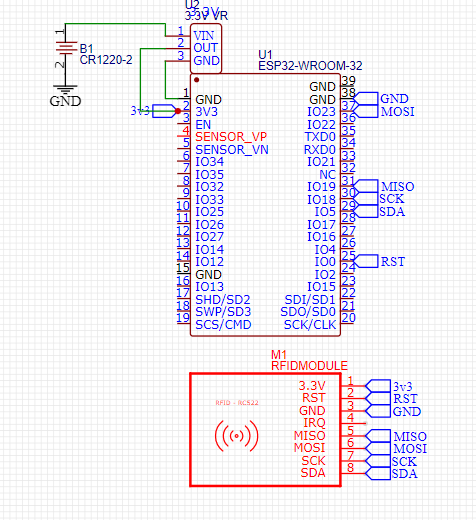
\includegraphics{assets/internalDiagram.png}
        \caption{Internt Diagram RFID-System}
    \end{figure}
    
    som det kan ses på skitsen har vi planlagt hvordan de forskellige komponenter skulle kobles sammen før vi gik i gang med at bestille delene hjem til produktet, selve udformningen og konstruktionen af produktet tog ikke særligt lang tid.
    den mest tidskrævende del af processen var at regne ud hvordan vi ville lave dør systemet, i starten overvejede vi at lave den som en knap på en app man kunne bruge til at låse døren op,
    men kom frem til at det var nemmere både produkt mæssigt men også for brugeren hvis døren benyttede sig af RFID da du der både har mulighed for at bruge en app på din Telefon, og et kort/chip til at låse døren op.


    \subsubsection{Kodegennemgang}

    Programmeringen af Esp'en viste sig også at være lidt af en udfordring da efter vi havde koblet alting sammen, kunne vi ikke få lov til at uploade kode til den. dette viste sig at tage noget tid at løse,
    så lad og gå igennem min process med at løse det.

    \begin{enumerate}    
        \item Vores første problem var at Arduino IDE ikke havde muligheden for at vælge den ESP32 som vi brugte, vi ledte en del tid efter nogen der havde en løsning, og kom frem til at det er fordi at den ESP32 vi bruger,
            ikke har sin egen kategori når du vælger hvilket board (Arduinoen) du bruger, men at den går ind under "Dev Module" kategorien.

        \item Det andet problem vi stødte på var at vi ikke kunne se den COM port (Communications/Serial Port) som min ESP32 kørte over, dette skyldes at vi manglede en driver der hedder "CP210x Universal Windows Driver",
            den gør det muligt for min computer at åbne de COM porte vi skulle benytte, og da den driver ikke var på min computer kunne vi ikke koble min ESP32 op.
        
        \item Det sidste problem vi stødte på var at selvom vi var koblet op til min ESP32 blev den ved med at give os fejlkoden "Wrong boot mode detected, device needs to be in download mode", dette forvirrede os lidt,
            da vi ikke var sikker på hvordan vi havde mulighed for at ændre hvilket boot mode min ESP32 var i. Dette problem var dog relativt nemt at løse da det viste sig at man skulle holde boot knappen på Esp'en nede,
            når man uploadede ting til den.
    \end{enumerate} 
        
        Efter vi havde overkommet de initiale udfordringer med Programmeringen, gik det faktisk overraskende nemt, det lykkedes os at finde et "Library" der havde eksempel kode der mindede meget om det vi havde brug for,
        til at få min scanner til at virke. \newline
        Se Bibliografi for kilder brugt til udvikling af ovenstående, \cite{ardDrive}, \cite{ardrfid}, \cite{ardProg}
 \newpage
    \section{Produktionsforberedelse}
    \subsection{Website-hosting}
        Der er to muligheder for hosting af websittet.
        Der er fjernhosting, hvor man lejer sig ind hos en central webserver, fx Vercel.
        Der er den anden mulighed, local hosting, hvor vi opstiller en decentral server på fx en skoles grund, hvor man så selv indkøber serverudstyr, veligeholder dette in-house eller igennem indkaldte teknikere\dots

        Det er gratis at anvende services som Vercel indtil et vist serverload opnås, hvorefter det koster penge. Jf. deres hjemmeside\cite{vercelprincing} kan hjemmesiden kun tigås en million gange per måned ved gratis abonnoment, ti millioner ved 20\$ per måned, men da vi forventer, at servicere et konservativt estimat på 50.000 gymnasieelever (baseret på Danmarks statistik \cite{ungudd}) om dagen, vil dette hurtigt blive overskredet, ergo er der tale om en unik dataaftale, hvorfor det nok bliver nok bliver markant dyre, men vil garanteret være billigere i sidste ende.

    \subsection{RFID-løsning /  låsemekanismesystem}
    \subsubsection{Fremtidig Plan}
    Da vi startede med projektet havde jeg meget høje forventninger til hvor meget jeg kunne nå at lave, selvom de ikke blev en realitet,
    har jeg stadigvæk tænkt mig at dele mine ideer. 
    \newline
    \newline
    Vores oprindelige ide var at bygge hele systemet, både med dørlukker, RFID scanner, og et komplet software system med database der ville havde givet elever og lærere
    mulighed for at booke lokaler og se hvem der var tilstede. Vores plan for at bygge døren var at købe en billig branddør,
    vi ville derefter havde opsæt en "skelet" dør (en dør som ikke sider fast i en væg), så vi ville have haft mulighed for at fremvise, hvordan produktet ville virke i praksis.
    vi havde tænkt os at bestille en elektronisk dørlukker, som vi ville havde koblet op til vores ESP32 i vores RFID kasse,
    vores plan var at trække 12v (Ledninger med 12 volts spænding) for at undgå højstrøms lovgivningen da 12v ledninger ikke indgår under denne lovgivning,
    dette ville havde signifikant sænket omkostninger for opsætning af systemet på skolen. Vi havde tænkt os at benytte et relæ (er et mekanisk kontakt),
    til at styre både dørlukkeren og den lås som vi ville havde sat i dørkarmen for at undgå kompliceret installation i dørene,
    også i forhold til tilfælde, hvor det kunne blive nødvendigt at udskifte døre. Dette ville også gøre designet mere simpelt og nemmere
    for os at konstruere. Desværre nåede vi aldrig så langt med vores planer, dette skyldes en del grunde men jeg har tænkt mig at nævne
    et par af de lidt større fejl og udfordringer der var skyld i at det ikke blev en realitet.
    \begin{enumerate}
        \item \textbf{For store ambitioner}\
            I starten af projektet havde vi en masse ideer som vi gerne ville føre til livs, dette resulterede i at størstedelen af vores tid blev
            brugt på at finde produkter og undersøge installations metoder ud fra vores meget store ambitioner, dette er jo nødvendigvis ikke en
            dårlig ting, men det var skyld i at vi i det første stykke tid ikke kom i gang med den den indledende konstruktion
            da vi var fokuseret på alle de mange ting vi ville. Da det så endeligt gik op for os at vi var ved at løbe tør for
            tid, havde vi allerede brugt en signifikant mængde af hele projekttiden.
        \item \textbf{For lidt prototyping}\
            Vi brugte rigtigt meget tid på at undersøge og prøve at udvikle et perfekt produkt før vi vidste om det overhovedet ville virke i
            praksis, hvis vi havde fokuseret mere på at lave nogen prototyper og eksperimentere i starten havde vi realiseret nogen af de
            design fejl der senere blev åbenlyse da vi lavede vores første prototype. Dette resulterede i at da vi endelig gik i gang med at
            konstruere og teste vores første prototype var vi nød til at gå tilbage til tegnebrættet og retænke vores design, hvilket
            resulterede i at der var mange ting vi ikke nåede i mål med da vi endeligt havde et fungerende design.
    \end{enumerate}
    
    \subsubsection{Produktion}
    bla bla

    \subsection{Teknologianalyse}
        Produktionen og veligholdesen af Lectio-rework applikation skal udliciteres til softwareudviklere fra Indien.
        Som udgangspunk skal hovedudviklingen af Lectio-reworket forgå i Danmark. I Danmark er infrastrukturen helt fin, og den er god nok i Indien til vores formål. Kulturen i Indien
        er meget inbydende til softwarevirksomheder som denne og arbejder gerne for et sådan projekt for den rette løn. Import / eksport til Kina ift. RFID-systemets 
        produktion er særligt nemt, da logistikinfrastrukturen er veletableret og -udbygget. Software kan let eksporteres fra Indien.
 \newpage
    
    \section{Evaluering, vurdering og konklusion \label{sec:konklusion}}
\subsection{Test af produkt}
Vi har testet produktet undervejs ved at udsættet testpersoner for produktet, hvorefter de har vurderet produktets æstetik og brugervenlighed rent kvalitativt, 
hvilket vi har taget til og ageret på.
\subsection{Teknologivurdering}
\subsubsection{Konsekvensvurdering}
Vi har lavet en konsekvensvurdering af Lectio, hvor vi er kommet frem til, at det er en ineffektiv IT-løsning, hvorefter vi har lavet et rework af dette med disse fejl og mangler rettet. 
Om hvorvidt vores applikationspakke bedre respekterer sine brugers tid, dvs. sparer den, vil kræve en kvantiativ undersøgelse, der først kan igangsættes, når produktet er blevet frigivet til flere mennesker. 
Envidere ville en kvalitativ undersøgelse skulle igangsættes for at vurdere om brugervenligheden er forbedret.
\subsection{Procesevaluering}
Vi har anvendt Gantt-diagram, skitser og systematiske metoder til at finde et fyldesgørende produkt til et relevant samfundsmæssigt problem, der vedrører vores studiemiljø. 
Det er gået udemærket, dog har vi skulle hugge en hæl og klippe en tå for at nå i mål--det er overordnet gået meget godt med den tid og de ressourcer, vi har haft til rådighed, dog var projektet en smule for ambitiøst. 
En anden gang vil vi anvende et andet markup-sprog til at holde styr og dokumentere vores projekt i, nemlig Org-Mode fremfor \LaTeX, da dette vil gøre, at vi bedre kan integrere kode i projektet samt fokusere mere på 
andre aspekter af projekter samt tillader os at anvende den overlegne Emacs til sit fulde potentiale.

\subsection{Konklusion}
All-in-all et vellykket projekt. \newpage
    \newpage
%% Back matter
    \printbibliography[heading=bibintoc,title={Bibliografi}]
    \begin{appendices} \newpage
        \section{Projektbeskrivelse \label{appendix:projektbeskrivelse}} \newpage
        \renewcommand*{\thepage}{A\arabic{page}}
        
\includepdf[pages=-,delta=5 5,frame=true,landscape=true,nup=1x2,pagecommand={\thispagestyle{plain}}]{appendix/Project description/project-description.pdf} \newpage
        \renewcommand*{\thepage}{\arabic{page}}
        \section{Logbog} \newpage
        \renewcommand*{\thepage}{B\arabic{page}}
        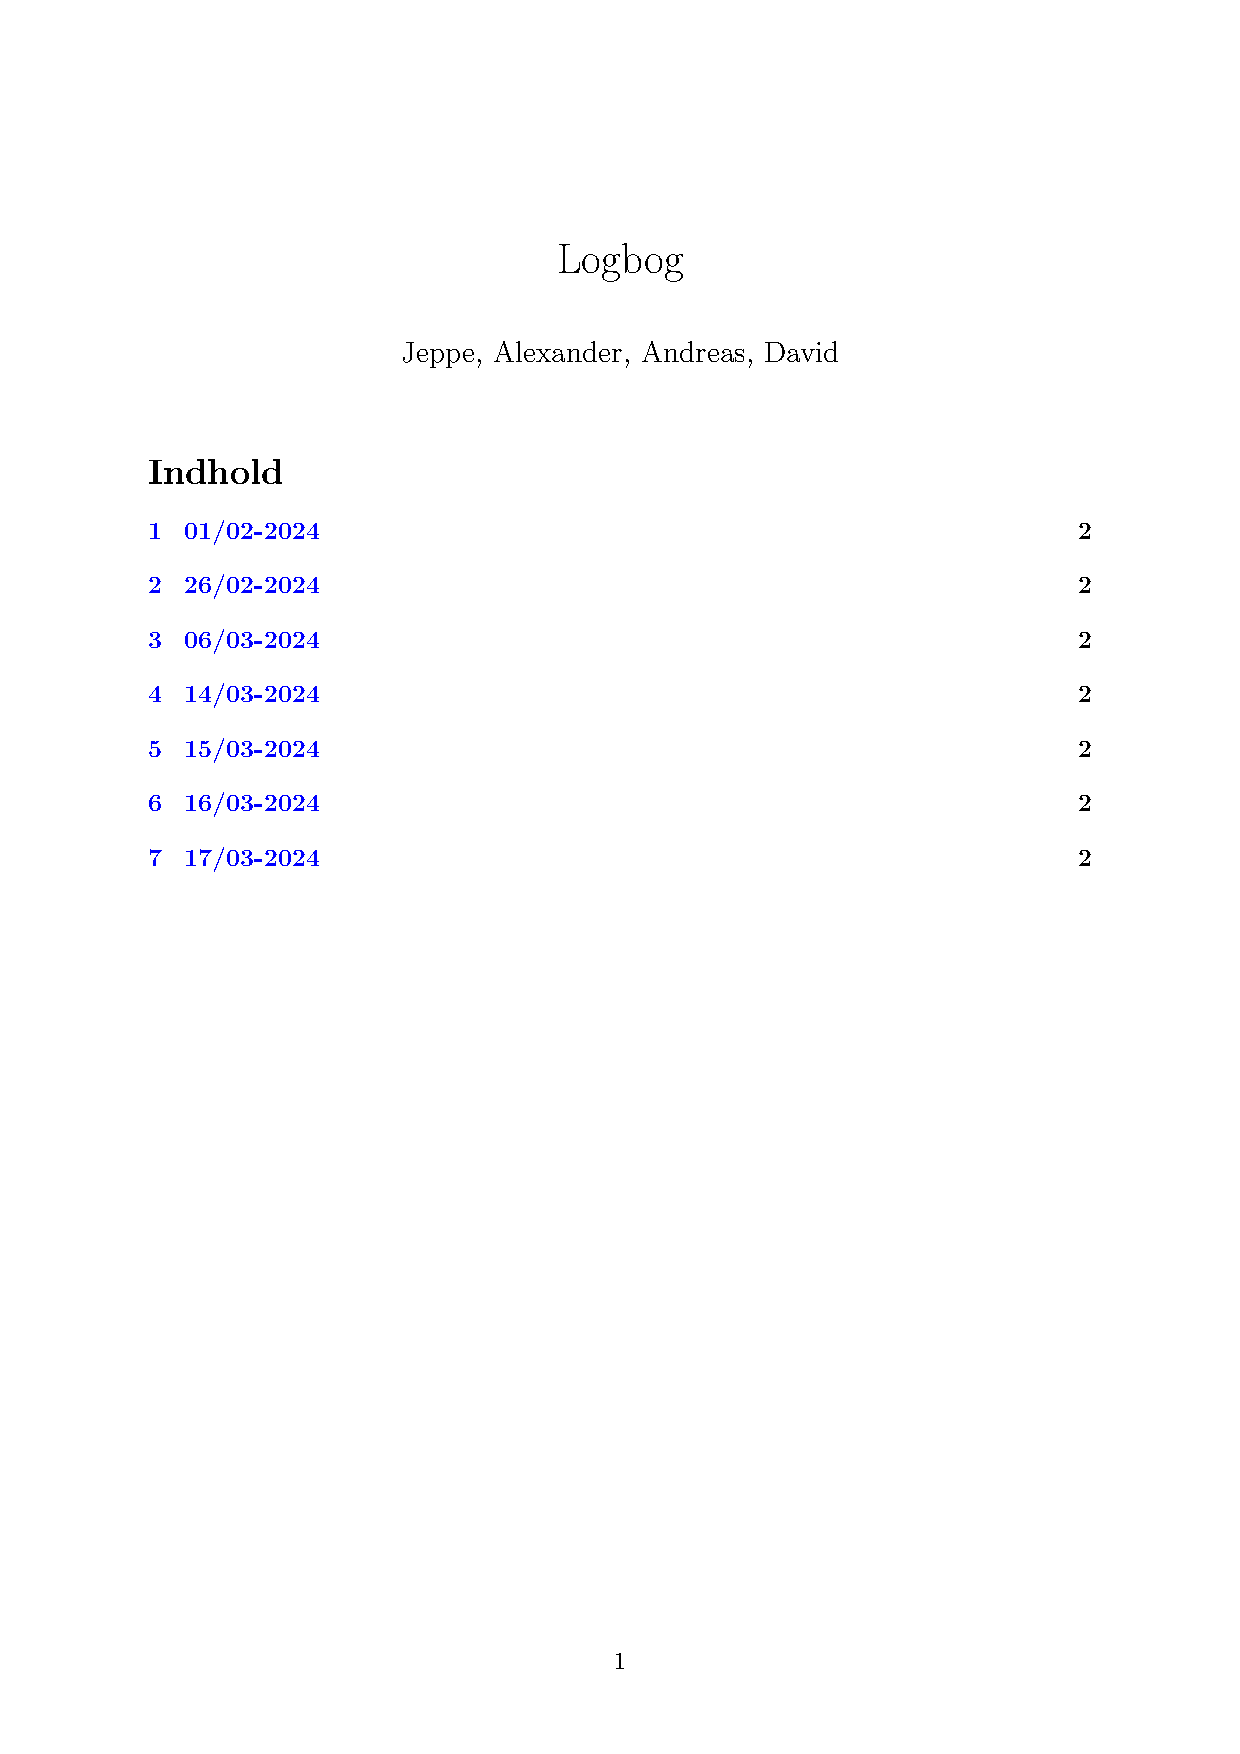
\includepdf[pages=-,delta=5 5,frame=true,landscape=true,nup=1x2,pagecommand={\thispagestyle{plain}}]{Log/log.pdf} \newpage
        \renewcommand*{\thepage}{\arabic{page}}

        \section{Arbejdsskitser \label{appendix:arbejdsskitser}} \newpage
        \renewcommand*{\thepage}{C\arabic{page}}
        \begin{figure}[H]
            \centering
            \resizebox{!}{10cm}{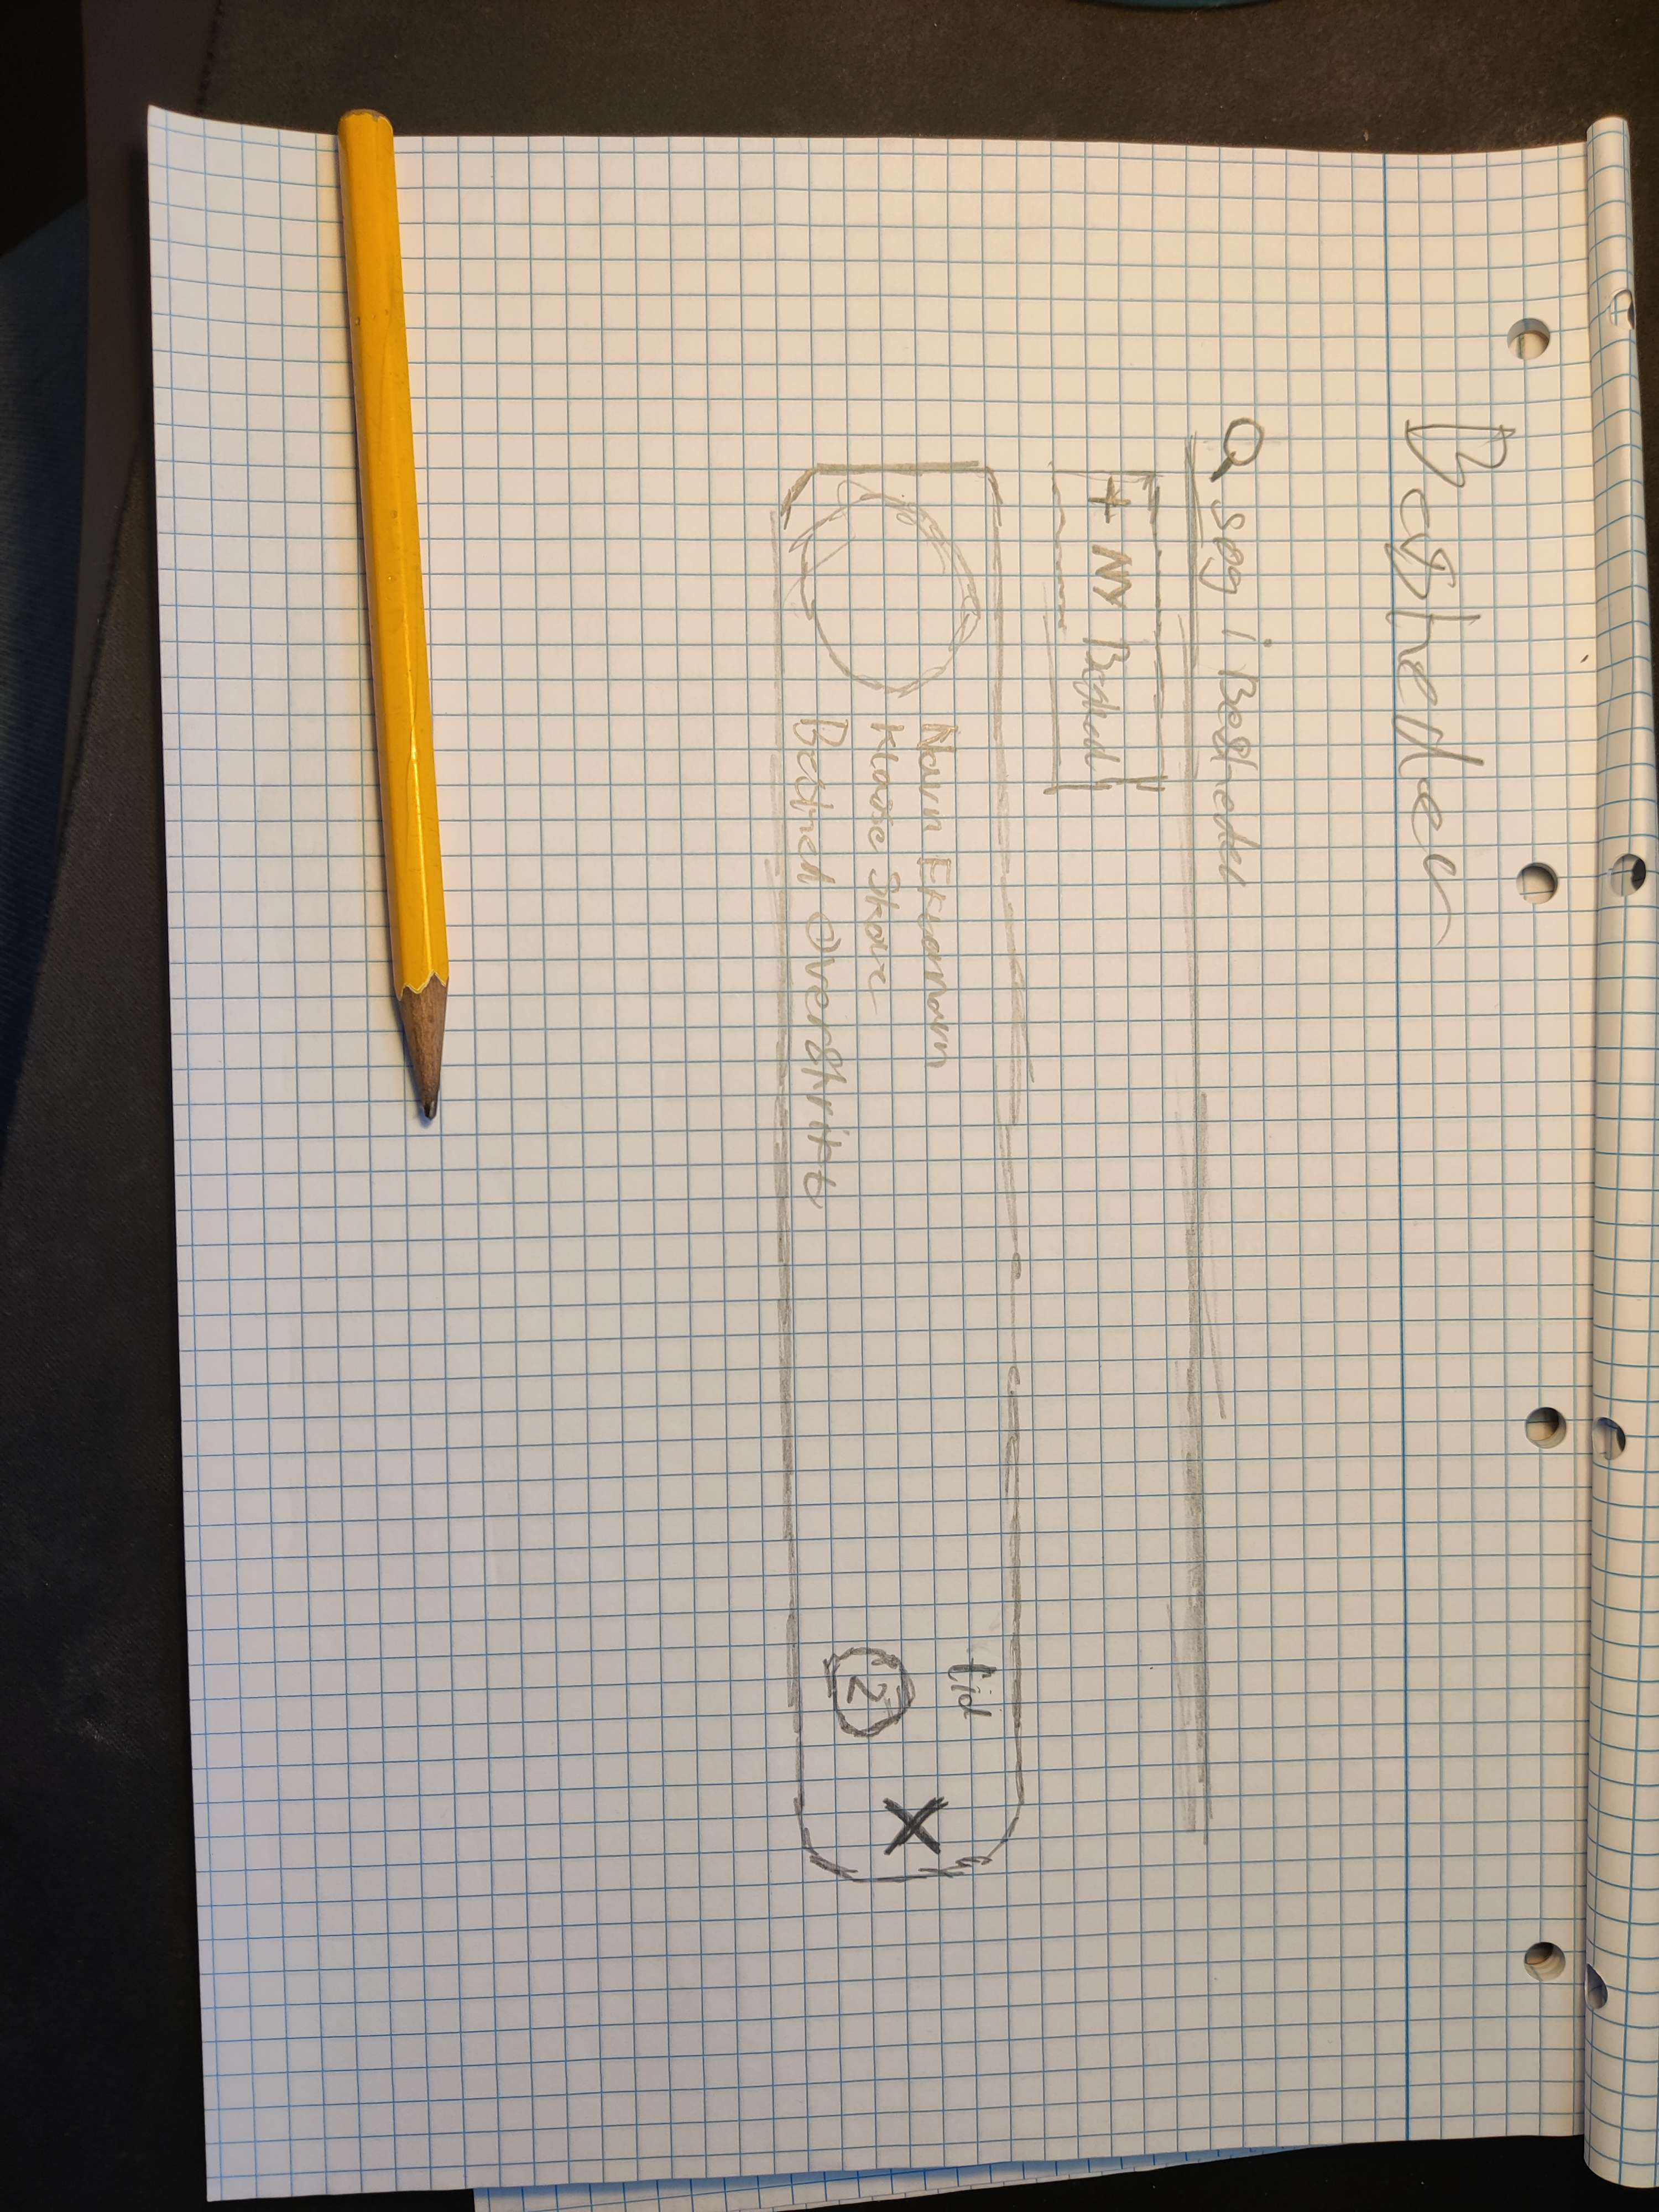
\includegraphics[angle=90]{assets/lectio_beskeder_skitse.jpg}} 
        \caption{Viser skitsen for lectiobesked-featuren}
        \end{figure}\newpage
        
        \begin{figure}[H]
            \centering
            \resizebox{!}{13cm}{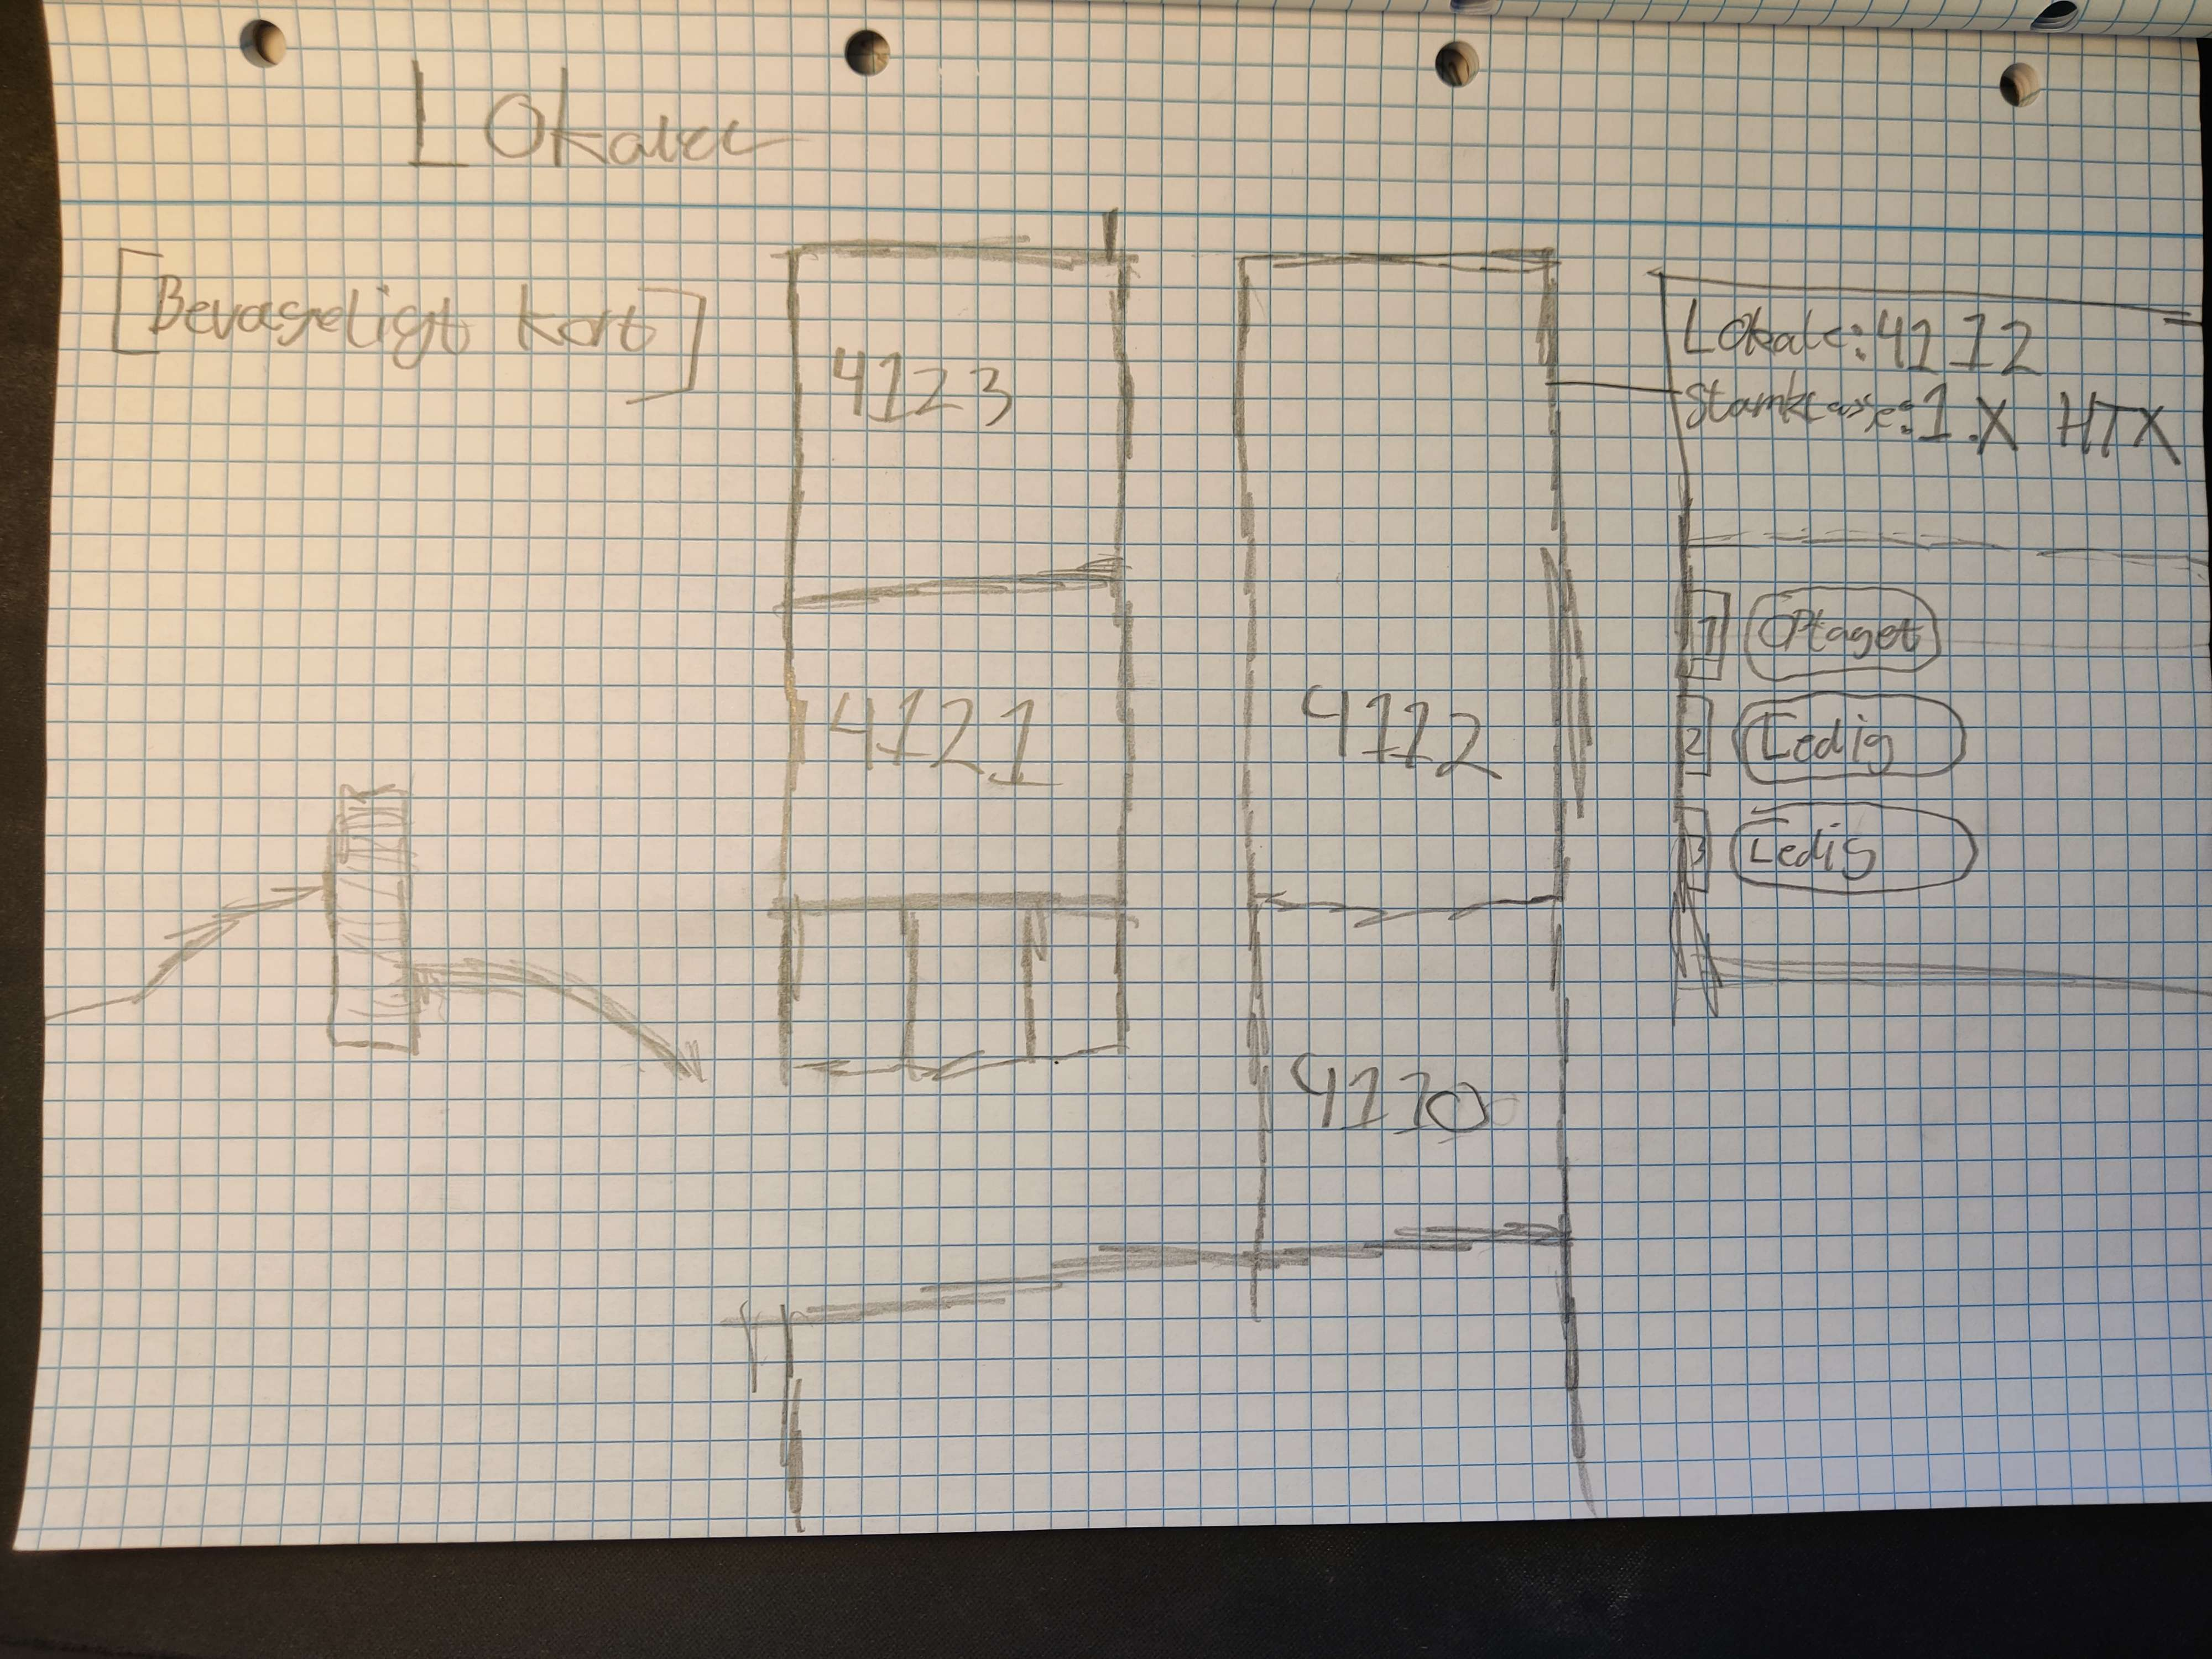
\includegraphics{assets/lectio_lokaler_skitse.jpg}}
            \caption{Viser skitsen for lectiolokalebooking-featuren}
        \end{figure}\newpage

        \begin{figure}[H]
            \centering
            \resizebox{!}{10cm}{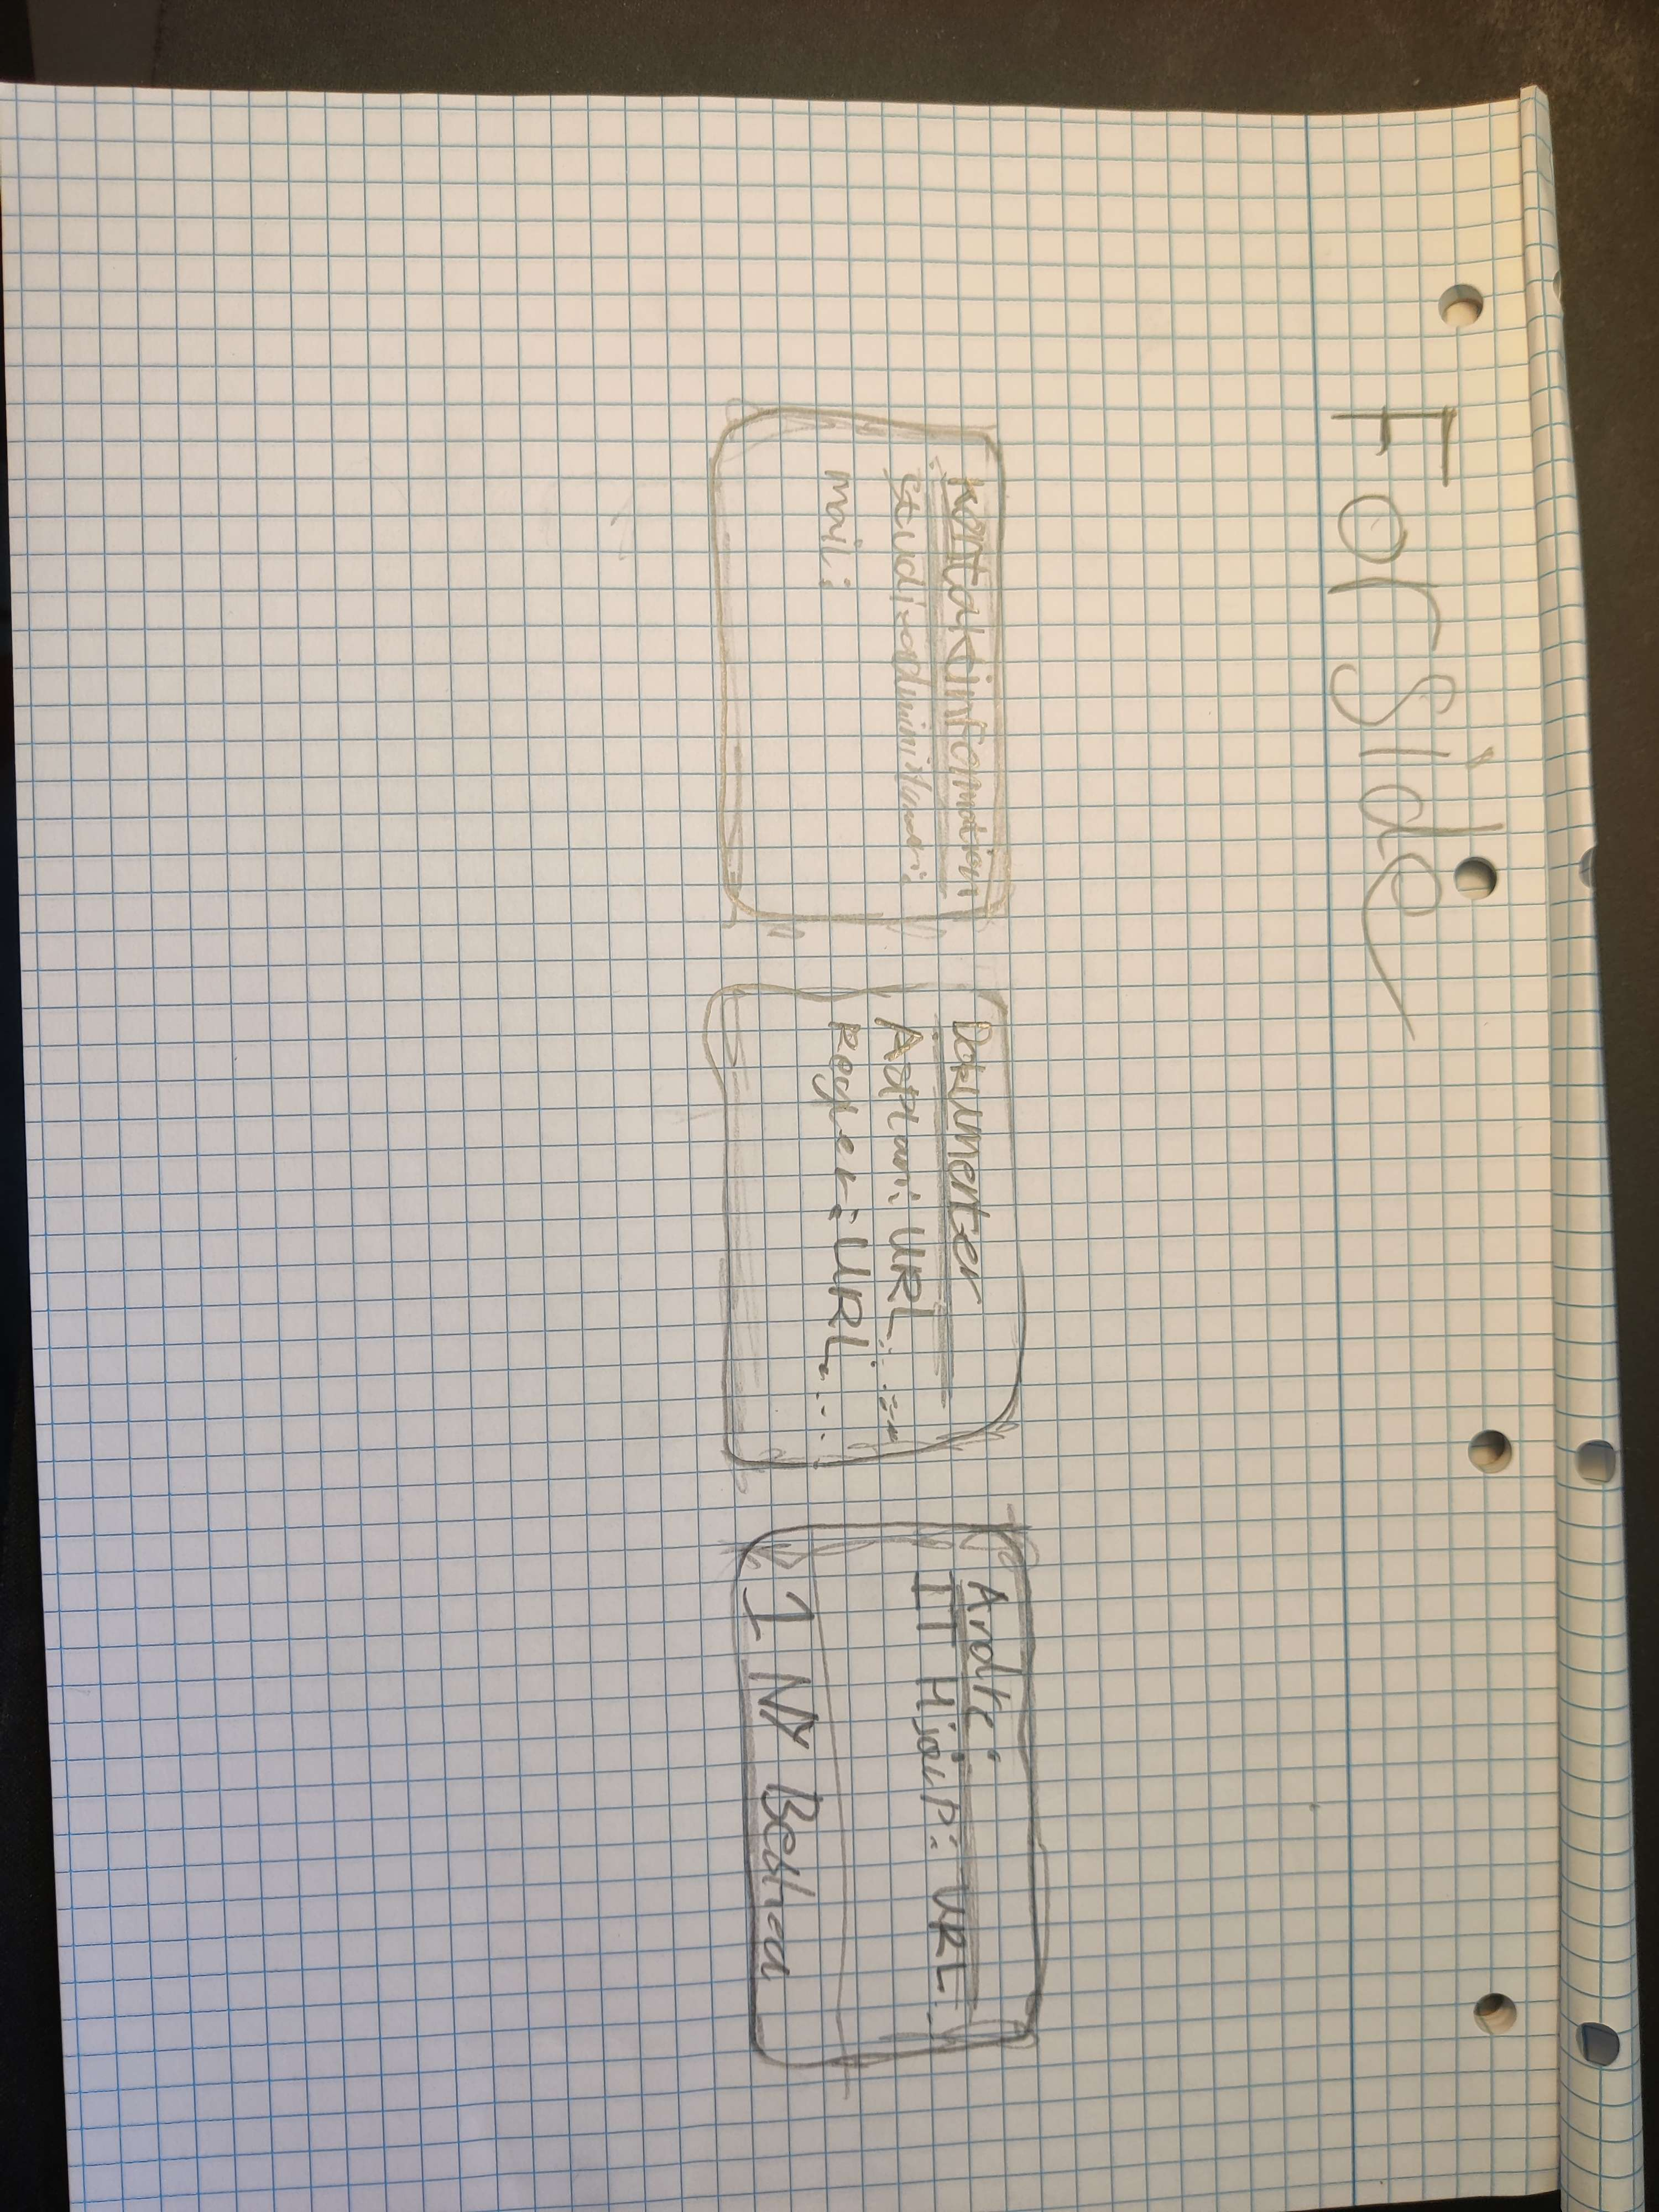
\includegraphics[angle =90]{assets/lectio_forside_skitse.jpg}}
            \caption{Viser skitsen for lectioskema-featuren}
        \end{figure}\newpage
        \renewcommand*{\thepage}{\arabic{page}}

        \section{Modulbrikkoden \label{appendix:modulbrikkode}} \newpage
        \renewcommand*{\thepage}{D\arabic{page}}
        \begin{lstlisting}[language=Javascript]
import './skema.css';
import { ChatBubbleOvalLeftIcon } from "@heroicons/react/24/outline";
import { PencilSquareIcon } from "@heroicons/react/24/outline";
import Link from 'next/link'


export default function skemaModule( args ) {

    if ( args.visibility == 'hide' ) {
        return (
            <div className="min-h-[88px]"></div>
        );
    } else {
        return (
        <Link href={`/skema/${args.id}`}>
        <div className="bg-[#9CCEFF] border-l-[10px] border-l-[#1E90FF] p-4 rounded-lg max-w-[275px] max-h-[88px] flex justify-between cursor-pointer hover:opacity-80 group">
            
            <div className="flex flex-col text-[#0D3F70] justify-center">
                <span className="font-bold text-xl">S 1x { args.subject }</span>
                <span>{ args.teacher }</span>
                <span>{ args.room }</span>
            </div>


        {/* Tooltip */}
        <div className='absolute'>
            <div className='max-w-[275px] flex flex-col flex-wrap mt-16'>
                <div>
                {(() => {
                    if ( args.note != '' ) {
                        return (
                            <span className='sidebar-tooltip group-hover:scale-100 relative left-[-30px]'><h1 className='font-black'>Note:</h1>&nbsp;<span>{ args.note }</span></span>
                            );
                        } else {
                            return (
                                ''
                                );
                            }
                })()} 
                </div>
                <div>
                {(() => {
                    if ( args.homework != '' ) {
                        return (
                            <span className='sidebar-tooltipH group-hover:scale-100 relative left-[-30px]'><h1 className='font-black'>Lektier:</h1>&nbsp;<span>{ args.homework }</span> </span>
                            );
                        } else {
                            return (
                                ''
                                );
                            }
                        })()} 
                </div>
            </div>
            </div>
            <div className="text-[#0D3F70] flex flex-row float-right">
                <div>
                    { (() => {
                        if ( args.note != '' ) {
                            return (
                                <span><ChatBubbleOvalLeftIcon className="h-5"/></span>
                                );
                            } else {
                                return (
                                    <span></span>
                                    );
                                }
                                
                            })()}
                </div>
                <div>
                    { (() => {
                        if ( args.homework != '' ) {
                            return (
                                <span><PencilSquareIcon className="h-5"/></span>
                                );
                            } else {
                                return (
                                    <span></span>
                            );
                        }
                        
                    })()}
                </div>
            </div>
        </div>
        </Link>
        );
    }
}
        \end{lstlisting} \newpage
        \section{Skemakomponentkode \label{appendix:SkemaModule}} \newpage
        \renewcommand*{\thepage}{D\arabic{page}}
        \begin{lstlisting}[language=Javascript]
<tbody>
                
{/* Module 1 */}
<tr>
    <td> <span className="h-[50px] bg-slate-300 py-10 px-2 rounded-e-md text-slate-600 font-bold">1.</span> </td>
    <td><SkemaModule subject={scheduleMon[0].subject} teacher={scheduleMon[0].teacher} room={scheduleMon[0].room} visibility={scheduleMon[0].visibility} note={scheduleMon[0].note} homework={scheduleMon[0].homework} id={scheduleMon[0].id}/></td>
    <td><SkemaModule subject={scheduleTue[0].subject} teacher={scheduleTue[0].teacher} room={scheduleMon[0].room} visibility={scheduleTue[0].visibility} note={scheduleTue[0].note} homework={scheduleTue[0].homework} id={scheduleTue[0].id}/></td>
    <td><SkemaModule subject={scheduleWed[0].subject} teacher={scheduleWed[0].teacher} room={scheduleWed[0].room} visibility={scheduleWed[0].visibility} note={scheduleWed[0].note} homework={scheduleWed[0].homework} id={scheduleWed[0].id}/></td>
    <td><SkemaModule subject={scheduleThu[0].subject} teacher={scheduleThu[0].teacher} room={scheduleThu[0].room} visibility={scheduleThu[0].visibility} note={scheduleThu[0].note} homework={scheduleThu[0].homework} id={scheduleThu[0].id}/></td>
    <td><SkemaModule subject={scheduleFri[0].subject} teacher={scheduleFri[0].teacher} room={scheduleFri[0].room} visibility={scheduleFri[0].visibility} note={scheduleFri[0].note} homework={scheduleFri[0].homework} id={scheduleFri[0].id}/></td>
</tr>

{/* Module 2 */}
<tr className="m-2">
    <td> <span className="h-[50px] bg-slate-300 py-10 px-2 rounded-e-md text-slate-600 font-bold">2.</span> </td>
    <td><SkemaModule subject={scheduleMon[1].subject} teacher={scheduleMon[1].teacher} room={scheduleMon[1].room} visibility={scheduleMon[1].visibility} note={scheduleMon[1].note} homework={scheduleMon[1].homework} id={scheduleMon[1].id} /></td>
    <td><SkemaModule subject={scheduleTue[1].subject} teacher={scheduleTue[1].teacher} room={scheduleTue[1].room} visibility={scheduleTue[1].visibility} note={scheduleTue[1].note} homework={scheduleTue[1].homework} id={scheduleTue[1].id} /></td>
    <td><SkemaModule subject={scheduleWed[1].subject} teacher={scheduleWed[1].teacher} room={scheduleWed[1].room} visibility={scheduleWed[1].visibility} note={scheduleWed[1].note} homework={scheduleWed[1].homework} id={scheduleWed[1].id} /></td>
    <td><SkemaModule subject={scheduleThu[1].subject} teacher={scheduleThu[1].teacher} room={scheduleThu[1].room} visibility={scheduleThu[1].visibility} note={scheduleThu[1].note} homework={scheduleThu[1].homework} id={scheduleThu[1].id} /></td>
    <td><SkemaModule subject={scheduleFri[1].subject} teacher={scheduleFri[1].teacher} room={scheduleFri[1].room} visibility={scheduleFri[1].visibility} note={scheduleFri[1].note} homework={scheduleFri[1].homework} id={scheduleFri[1].id} /></td>
</tr>

{/* Module 3 */}
<tr>
<td> <span className="h-[50px] bg-slate-300 py-10 px-2 rounded-e-md text-slate-600 font-bold">3.</span> </td>
    <td><SkemaModule subject={scheduleMon[2].subject} teacher={scheduleMon[2].teacher} room={scheduleMon[2].room} visibility={scheduleMon[2].visibility} note={scheduleMon[2].note} homework={scheduleMon[2].homework} id={scheduleMon[2].id} /></td>
    <td><SkemaModule subject={scheduleTue[2].subject} teacher={scheduleTue[2].teacher} room={scheduleTue[2].room} visibility={scheduleTue[2].visibility} note={scheduleTue[2].note} homework={scheduleTue[2].homework} id={scheduleTue[2].id} /></td>
    <td><SkemaModule subject={scheduleWed[2].subject} teacher={scheduleWed[2].teacher} room={scheduleWed[2].room} visibility={scheduleWed[2].visibility} note={scheduleWed[2].note} homework={scheduleWed[2].homework} id={scheduleWed[2].id} /></td>
    <td><SkemaModule subject={scheduleThu[2].subject} teacher={scheduleThu[2].teacher} room={scheduleThu[2].room} visibility={scheduleThu[2].visibility} note={scheduleThu[2].note} homework={scheduleThu[2].homework} id={scheduleThu[2].id} /></td>
    <td><SkemaModule subject={scheduleFri[2].subject} teacher={scheduleFri[2].teacher} room={scheduleFri[2].room} visibility={scheduleFri[2].visibility} note={scheduleFri[2].note} homework={scheduleFri[2].homework} id={scheduleFri[2].id} /></td>
</tr>

{/* Module 4 */}
<tr>
<td> <span className="h-[50px] bg-slate-300 py-10 px-2 rounded-e-md text-slate-600 font-bold">4.</span> </td>
    <td><SkemaModule subject={scheduleMon[3].subject} teacher={scheduleMon[3].teacher} room={scheduleMon[3].room} visibility={scheduleMon[3].visibility} note={scheduleMon[3].note} homework={scheduleMon[3].homework} id={scheduleMon[3].id} /></td>
    <td><SkemaModule subject={scheduleTue[3].subject} teacher={scheduleTue[3].teacher} room={scheduleTue[3].room} visibility={scheduleTue[3].visibility} note={scheduleTue[3].note} homework={scheduleTue[3].homework} id={scheduleTue[3].id} /></td>
    <td><SkemaModule subject={scheduleWed[3].subject} teacher={scheduleWed[3].teacher} room={scheduleWed[3].room} visibility={scheduleWed[3].visibility} note={scheduleWed[3].note} homework={scheduleWed[3].homework} id={scheduleWed[3].id} /></td>
    <td><SkemaModule subject={scheduleThu[3].subject} teacher={scheduleThu[3].teacher} room={scheduleThu[3].room} visibility={scheduleThu[3].visibility} note={scheduleThu[3].note} homework={scheduleThu[3].homework} id={scheduleThu[3].id} /></td>
    <td><SkemaModule subject={scheduleFri[3].subject} teacher={scheduleFri[3].teacher} room={scheduleFri[3].room} visibility={scheduleFri[3].visibility} note={scheduleFri[3].note} homework={scheduleFri[3].homework} id={scheduleFri[3].id} /></td>
</tr>

{/* Module 5 */}
<tr>
<td> <span className="h-[50px] bg-slate-300 py-10 px-2 rounded-e-md text-slate-600 font-bold">5.</span> </td>
    <td><SkemaModule subject={scheduleMon[4].subject} teacher={scheduleMon[4].teacher} room={scheduleMon[4].room} visibility={scheduleMon[3].visibility} note={scheduleMon[4].note} homework={scheduleMon[4].homework} id={scheduleMon[4].id} /></td>
    <td><SkemaModule subject={scheduleTue[4].subject} teacher={scheduleTue[4].teacher} room={scheduleTue[4].room} visibility={scheduleTue[4].visibility} note={scheduleTue[4].note} homework={scheduleMon[4].homework} id={scheduleTue[4].id} /></td>
    <td><SkemaModule subject={scheduleWed[4].subject} teacher={scheduleWed[4].teacher} room={scheduleWed[4].room} visibility={scheduleWed[4].visibility} note={scheduleWed[4].note} homework={scheduleTue[4].homework} id={scheduleWed[4].id} /></td>
    <td><SkemaModule subject={scheduleThu[4].subject} teacher={scheduleThu[4].teacher} room={scheduleThu[4].room} visibility={scheduleThu[4].visibility} note={scheduleThu[4].note} homework={scheduleWed[4].homework} id={scheduleThu[4].id} /></td>
    <td><SkemaModule subject={scheduleFri[4].subject} teacher={scheduleFri[4].teacher} room={scheduleFri[4].room} visibility={scheduleFri[4].visibility} note={scheduleFri[4].note} homework={scheduleFri[4].homework} id={scheduleFri[4].id} /></td>
</tr>

{/* Module 6 */}
<tr>
<td> <span className="h-[50px] bg-slate-300 py-10 px-2 rounded-e-md text-slate-600 font-bold">6.</span> </td>
    <td><SkemaModule subject={scheduleMon[5].subject} teacher={scheduleMon[5].teacher} room={scheduleMon[5].room} visibility={scheduleMon[5].visibility} note={scheduleMon[5].note} homework={scheduleMon[5].homework} id={scheduleMon[5].id} /></td>
    <td><SkemaModule subject={scheduleTue[5].subject} teacher={scheduleTue[5].teacher} room={scheduleTue[5].room} visibility={scheduleTue[5].visibility} note={scheduleTue[5].note} homework={scheduleTue[5].homework} id={scheduleTue[5].id} /></td>
    <td><SkemaModule subject={scheduleWed[5].subject} teacher={scheduleWed[5].teacher} room={scheduleWed[5].room} visibility={scheduleWed[5].visibility} note={scheduleWed[5].note} homework={scheduleWed[5].homework} id={scheduleWed[5].id} /></td>
    <td><SkemaModule subject={scheduleThu[5].subject} teacher={scheduleThu[5].teacher} room={scheduleThu[5].room} visibility={scheduleThu[5].visibility} note={scheduleThu[5].note} homework={scheduleThu[5].homework} id={scheduleThu[5].id} /></td>
    <td><SkemaModule subject={scheduleFri[5].subject} teacher={scheduleFri[5].teacher} room={scheduleFri[5].room} visibility={scheduleFri[5].visibility} note={scheduleFri[5].note} homework={scheduleFri[5].homework} id={scheduleFri[5].id} /></td>
</tr>

{/* Module 7 */}
<tr>
<td> <span className="h-[50px] bg-slate-300 py-10 px-2 rounded-e-md text-slate-600 font-bold">7.</span> </td>
    <td><SkemaModule subject={scheduleMon[6].subject} teacher={scheduleMon[6].teacher} room={scheduleMon[6].room} visibility={scheduleMon[6].visibility} note={scheduleMon[6].note} homework={scheduleMon[6].homework} id={scheduleMon[6].id} /></td>
    <td><SkemaModule subject={scheduleTue[6].subject} teacher={scheduleTue[6].teacher} room={scheduleTue[6].room} visibility={scheduleTue[6].visibility} note={scheduleTue[6].note} homework={scheduleTue[6].homework} id={scheduleTue[6].id} /></td>
    <td><SkemaModule subject={scheduleWed[6].subject} teacher={scheduleWed[6].teacher} room={scheduleWed[6].room} visibility={scheduleWed[6].visibility} note={scheduleWed[6].note} homework={scheduleWed[6].homework} id={scheduleWed[6].id} /></td>
    <td><SkemaModule subject={scheduleThu[6].subject} teacher={scheduleThu[6].teacher} room={scheduleThu[6].room} visibility={scheduleThu[6].visibility} note={scheduleThu[6].note} homework={scheduleThu[6].homework} id={scheduleThu[6].id} /></td>
    <td><SkemaModule subject={scheduleFri[6].subject} teacher={scheduleFri[6].teacher} room={scheduleFri[6].room} visibility={scheduleFri[6].visibility} note={scheduleFri[6].note} homework={scheduleFri[6].homework} id={scheduleFri[6].id} /></td>
</tr>
</tbody>
        \end{lstlisting} \newpage
        \section{Datahåndteringssystem \label{appendix:datahåndteringssystem}} \newpage
        \renewcommand*{\thepage}{F\arabic{page}}
        \begin{lstlisting}[language=Javascript]
export default function skema() {
const weekNumbers = ["29/4", "30/4", "1/5", "2/5", "3/5"];


const today = new Date();
const month = today.getMonth()+1;
const year = today.getFullYear();
const date = today.getDate();
const currentDate = month + "/" + date + "/" + year;

const currentFormattedDate = month + "-" + date + "-" + year; 

const weekDate = date + "/" + month;

var currentWeekNumber = require('current-week-number');


return (
    <div className="px-10">
        <Link href={`/${scheduleMon[1].subject + '-' + currentFormattedDate}`}></Link>
        
        <div className="container">
            <div className="w-[80vw] h-[100vh] py-10">
                <div className="w-full flex justify-center font-bold bg-white py-2">
                    <h1> Uge { currentWeekNumber(currentDate) } - { year }</h1>
                </div>
                <table className="w-full h-full bg-white">
                    <thead>
                        <tr className="h-20">
                            <th></th>
                            <th> 
{ (() => {
        if (weekNumbers[0] == weekDate) {
            return (
                <span className="px-10 p-4 rounded-xl bg-[#1E90FF] text-white font-normal">Mandag <strong>{ weekNumbers[0] }</strong></span> 
            );
        } else {
            return (
                <span className="px-10 p-4 rounded-xl bg-slate-200 font-normal">Mandag <strong>{ weekNumbers[0] }</strong></span>
            );
        }

    })()}
</th>
<th> 
{ (() => {
    if (weekNumbers[1] == weekDate) {
        return (
            <span className="px-10 p-4 rounded-xl bg-[#1E90FF] text-white font-normal">Tirsdag <strong>{ weekNumbers[1] }</strong></span> 
        );
    }   else {
        return (
            <span className="px-10 p-4 rounded-xl bg-slate-200 font-normal">Tirsdag <strong>{ weekNumbers[1] }</strong></span> 
        );
    }
}) ()}
</th>
<th> 
{ (() => {
    if (weekNumbers[2] == weekDate) {
        return (
            <span className="px-10 p-4 rounded-xl bg-[#1E90FF] text-white font-normal">Onsdag <strong>{ weekNumbers[2] }</strong></span> 
        );
    }   else {
        return (
            <span className="px-10 p-4 rounded-xl bg-slate-200 font-normal">Onsdag <strong>{ weekNumbers[2] }</strong></span> 
        );
    }
}) ()}
</th>
<th> 
{ (() => {
    if (weekNumbers[3] == weekDate) {
        return (
            <span className="px-10 p-4 rounded-xl bg-[#1E90FF] text-white font-normal">Torsdag <strong>{ weekNumbers[3] }</strong></span> 
        );
    }   else {
        return (
            <span className="px-10 p-4 rounded-xl bg-slate-200 font-normal">Torsdag <strong>{ weekNumbers[3] }</strong></span> 
        );
    }
}) ()}
</th>
<th> 
{ (() => {
    if (weekNumbers[4] == weekDate) {
        return (
            <span className="px-10 p-4 rounded-xl bg-[#1E90FF] text-white font-normal">Fredag <strong>{ weekNumbers[4] }</strong></span> 
        );
    }   else {
        return (
            <span className="px-10 p-4 rounded-xl bg-slate-200 font-normal">Fredag <strong>{ weekNumbers[4] }</strong></span> 
        );
    }
}) ()}
                            </th>
                        </tr>
                    </thead>
        \end{lstlisting} \newpage

        \section{Eksempel på beskedfunktionalitet} \newpage
        \renewcommand*{\thepage}{G\arabic{page}}
        \begin{landscape}
        \begin{figure}[H]
        \centering
        \resizebox{\columnwidth}{!}{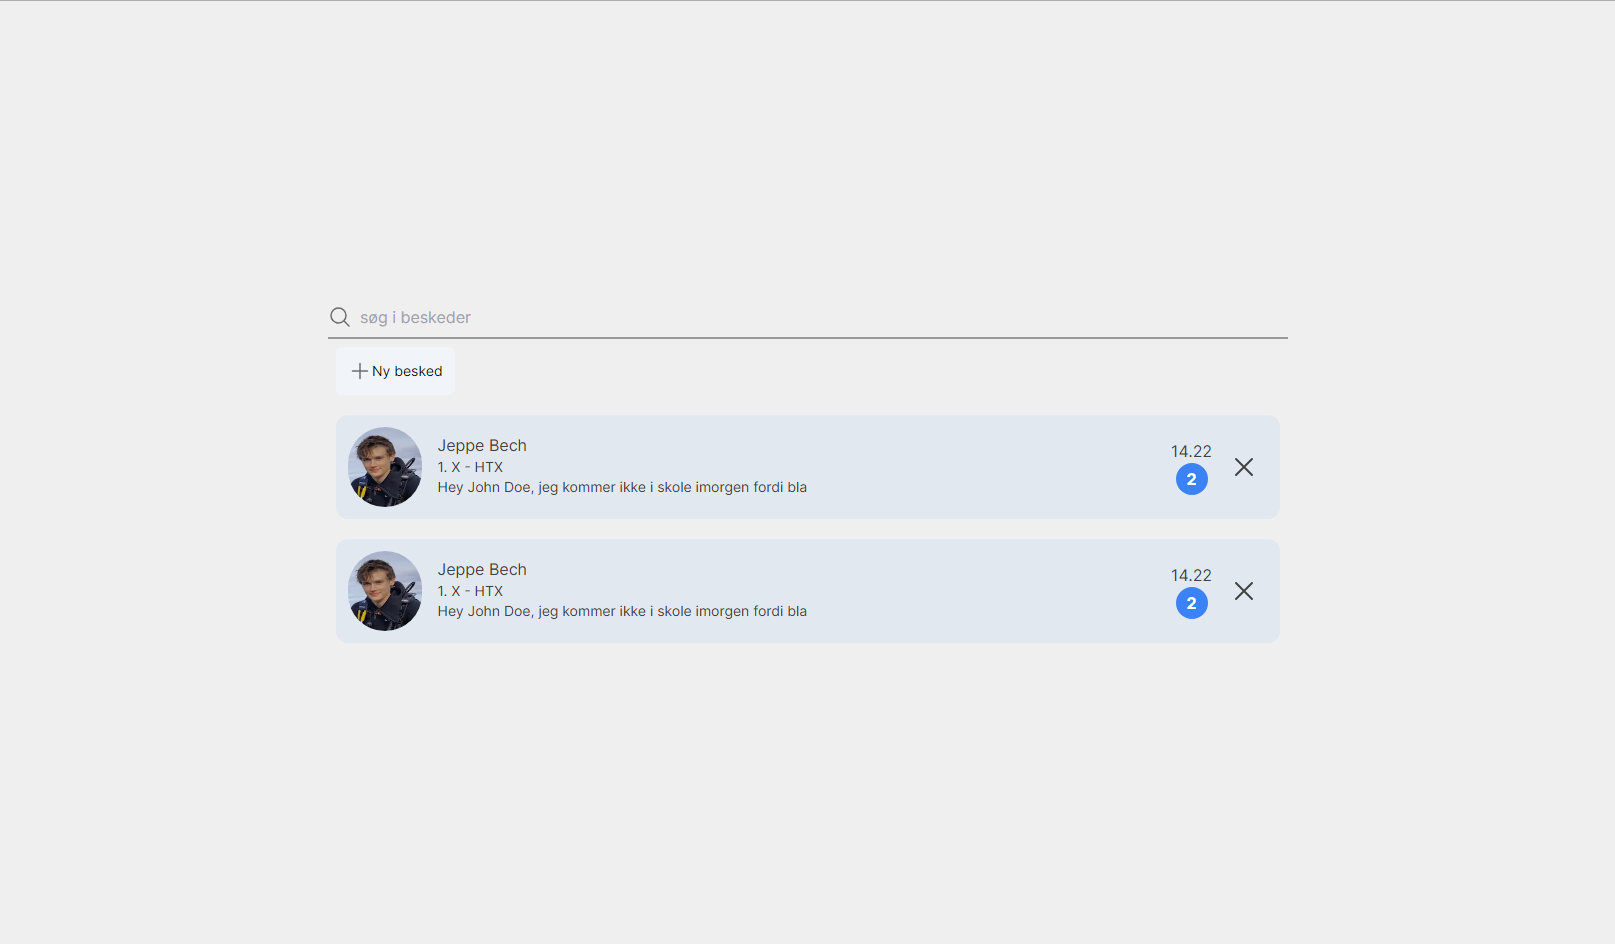
\includegraphics{assets/beskeder.png}}
        \end{figure}
        \end{landscape}
    
    \end{appendices}
\end{document}
